\documentclass[12pt, journal,compsoc]{./IEEEtran}

\usepackage[a4paper, tmargin=0.115\paperheight, bmargin=0.115\paperheight]{geometry} %margins
%\usepackage{parskip}

\usepackage{url}
\usepackage{amsmath}
\usepackage{amsfonts}
\usepackage{graphicx}
\usepackage[utf8]{inputenc}
\usepackage{subcaption}
\usepackage{csquotes}
\usepackage{pdfpages}
\usepackage{tabularx}
\usepackage{booktabs,fancyhdr}
%\usepackage{makecell}

\usepackage{nameref}

\usepackage{xcolor}
\usepackage{soulutf8}

\usepackage{float}


\newcommand{\changeRemove}[1]{}
\newcommand{\changeAdd}[1]{#1}


\usepackage[swedish]{babel}
\setlength{\parindent}{1cm}
\setlength{\parskip}{0mm}


\selectlanguage{swedish}

\usepackage[backend=bibtex, citestyle=ieee, bibstyle=ieee]{biblatex}
\addbibresource{ref.bib}

\begin{document}
\sloppy



% \title{User Experience på Amazing Leaders prototyp}


% \author{
% 	\changeAdd{Kandidatarbete}\\
% 	~Anna~Zakipour,
%     ~Leila~Englund\\
%     KTH - Royal Institue of Technology, Stockholm
%     \thanks{Handledare på KTH - Patric Dahlqvist}
%     \thanks{Handledare på VNTRS}
%     \thanks{Handledare på Amazing Leaders}}


% The paper headers
% \markboth{Kandidatarbete, ICT II143X - 2018 - KTH}%
% {}

% \IEEEtitleabstractindextext{
% \begin{abstract} 
%User Experience (UX) is a popular term within the development industry as well as the research field human-computer interaction (HCI). The purpose of this thesis is to examine UX and to test a prototype to be able to compare UX in theory and practice. To
%find out what the UX encompasses around the prototype different UX methods were used. This surrounds a literature study, a qualitative case study where focus groups was used and finally a quantitative study with a questionnare. The study was done at the company VNTRS where the customer is Amazing Leaders. Based on the findings in both the survey and the literature study, a case study about UX in practice was constructed.  The case study was done with Amazing Leaders, with focus groups where the method was semi-structured
%interviews. The result was mainly about... %Based on the categories and terms that were identifiable in the interviews, % the literature study was extended and deepened in those specific areas. 
%The respondents in the survey represented the end-user and people intressted of becoming more EQ-smart.
%We see UX as a way of working it is in theory described as user-centered and with a number of sub-processes or components that we describe: personas, scenarios, prototypes, evaluation and testing with end users and experts. The work should also be performed iteratively.
%The empirical data indicated that there is one (singular) established way of working, or a framework, that is called UX, in practice it means that you work user-centered. 
%To achieve a good user experience, certain tools are used or certain processes are performed; personas, i.e. mappings of end-user groups – with backgrounds, pre-conditions, needs and so on – through observation and interviews. Prototypes are developed that meet the needs identified in the personas, and the prototype is tested and evaluated with end users, and the process is repeated until the prototype is
%accepted. In this thesis this is done in practice where the result show what needs to be improved. The study’s respondents showed that.....
%\end{abstract}

% \begin{IEEEkeywords}
% VNTRS, Amazing Leaders, UX, EQ
% \end{IEEEkeywords}
%}

% make the title area
%\maketitle

\newpage
\input{sections/0-cover}

\newpage \thispagestyle{empty}

\section*{Abstract}




\newpage \thispagestyle{empty}

\section*{Sammanfattning}

\newpage 
\input{sections/1.2-Inneh_llsf_rteckning}
\tableofcontents 
\addtocontents{toc}{\protect\thispagestyle{empty}}

\newpage
\clearpage
\setcounter{page}{1}
\section{Inledning}
Internets utveckling är en av de starkaste krafterna som har förändrat vår värld de senaste två decennierna\cite{Davidsson2017Svenskarna2017}. Dagligen möts vi av olika webbapplikationer som vi interagerar med, både i arbetslivet och på fritiden\cite{Six2011TheUXmatters}. Således är det viktigt att användaren kan interagera med applikationen på ett så enkelt och bra sätt som möjligt \cite{Six2011TheUXmatters}. För att detta ska ske är en av grundprinciperna att sätta användaren i fokus\cite{Six2011TheUXmatters}. Genom att ta reda på vad användaren tycker och vad som kan förbättra användarupplevelsen skapas ett större värde för applikationen\cite{Rodden2010MeasuringApplications}. Oavsett om applikationen ska användas av privatpersoner eller internt på ett företag ger information om användarupplevelsen en viktig och värdefull åsikt som kan bidra till förbättringar \cite{Rodden2010MeasuringApplications}.
\newline

\parindent
\parskip

\subsection{Bakgrund}
Datorsystem är en typ av interaktivt system och karakteriseras av ett signifikant antal interaktioner mellan människa och dator \cite{InteractiveDictionary}. Interaktiva system är något som behöver vara användbart, lättförståeligt och som får användaren till fortsatt användning\cite{May2012ApplyingApp}. Interaktiva system är således något som måste utgå från människocentrerad design\cite{Human-CenteredStudio}. Människocentrerad design utgår från fysiska och psykiska behov hos mänskliga användare\cite{Millot2014Human-CenteredDesign}. Människocentrerad design blandas ofta ihop med termen användarcentrerad design\cite{Abras2004User-CenteredDesign}. Användarcentrerad design fokuserar på en djupare analys av målgruppen, specifika egenskaper och specifika egenskaper hos målgruppen, denna typ av design är något som fokuserats på i denna rapport.
\newline

Människa- datorinteraktion (MDI) är ett forskningsområde som studerar interaktionen mellan människa och dator\cite{Blanton2009Human-ComputerInteraction}. Forskningsområdet etablerades på tidigt 60-tal men det var inte förrän på 80-talet som termen Människa- datorinteraktion fick sin spridning\cite{Myers1998ATechnology}. Idag ses MDI och dess begrepp som en nödvändighet för att utforma interaktiva system\cite{TheCambridge}. 
\newline

Ett nyckelkoncept inom MDI är något som kallas \textit{användbarhet}\cite{Myers1998ATechnology}. Begreppet är en mätning på hur väl användaren kan interagera med eller använda ett system \cite{Blanton2009Human-ComputerInteraction}. För att uppnå en god användbarhet krävs det att man arbetar med människocentrerad design där man arbetar med principer som effektivitet, minnesvärdighet och tillfredsställelse\cite{Blanton2009Human-ComputerInteraction}. 
\newline

Ett annat centralt begrepp som etablerat sig inom MDI på senare tid är User Experience (UX). User Experience direkt översatt till svenska är \textit{användarupplevelse}. UX är alla aspekter av slutanvändarens interaktion med företaget, dess tjänster och dess produkter enligt Norman\cite{NormanTheUX}, forskare inom människa- datorinteraktion. UX kan appliceras inom alla branscher, produkter eller tjänster, på alla lösningar där användaren är i fokus\cite{Axbom2013JagAxbom}. UX som forskningsområde syftar till användarens totala upplevelse av en produkt eller tjänst\cite{20Mastery}. 
\newline

Då teknik har blivit så pass etablerat i vårt samhälle där interaktiva system har blivit en stor del av människans vardag är det viktigt att interaktionen med systemen sker på bästa möjliga sätt \cite{Six2011TheUXmatters}. Den största utmaningen vad det gäller denna utveckling är hur man får användaren till fortsatt användning\cite{SafferCreatingDevices}. Det är många faktorer som spelar in vid utveckling av ett lyckat interaktivt system. Bland dessa faktorer spelar användbarhet och UX en stor roll\cite{SafferCreatingDevices}. På endast ett fåtal år har samsynen på UX blivit mer uppmärksammad där man har fått större förståelse för att upplevelsen för användaren kan gå förlorad under projektets olika stadier fram till att produkten är klar\cite{BrannmarkGustavJansaterHandledareInstitutionenInformatik}. Genom att utveckla systemen utefter ett människocentrerat perspektiv är chansen större att systemet tillfredsställer användarens behov och bidrar till fortsatt användning\cite{May2012ApplyingApp}. 

%Denna rapport kommer att utgå från ett teoretiskt ramverk för UX som metodik för att beskriva olika dimensioner av användarupplevelsen. Detta ramverk är framtaget av Marc Hassenzahl \cite{Hassenzahl2001TheAppealingness} där målet är att förstå vilken kategori slutanvändaren anser vara både viktigast för användarupplevelsen men också som en kartläggning för utvärdering av användarupplevelsen. Kategoriseringen som tagits fram och som även används i denna rapport är: \enquote{Attraktivitet, Tydlighet, Stimuli, Pålitlighet och Effektivitet} \cite{Laugwitz2008ConstructionQuestionnaire}.

\subsection{Uppdragsarbetet}
Kandidatarbetet utförs tillsammans med \textit{VNTRS} \cite{VNTRSVNTRSAB} åt \textit{Amazing Leaders}\cite{AmazingOrganisationsutveckling}. VNTRS är ett konsultbolag som startades år 2016 av fyra management konsulter. VNTRS har i nuläget (2018) 21 anställda som arbetar med att hjälpa företag att bygga innovativa digitala produkter. VNTRS arbetar bland annat tillsammans med Amazing Leaders, som är en av deras uppdragsgivare.
\newline
\parindent
\parskip

Amazing Leaders är en organisation som grundades av tidigare industriledare som nu coachar och utbildar sina kunder. Utbildningens syfte är att öka ledareffektivitet. Ledareffektiviteten utvecklas med hjälp av metoder inom forskningsområdet EQ (Emotional Quotient / emotionell kvot) och coachningen går ut på att höja denna kvot. Amazing Leaders avser i framtiden att erbjuda utbildningsprogram där programmen delvis utförs digitalt via en app, eller där digitala appar finns tillgängliga som hjälpmedel under programmets gång. VNTRS och Amazing Leaders samarbetar idag för att uppnå denna vision. 
\newline
\parindent
\parskip

Som del av utvecklingsarbetet för att uppnå deras mål har VNTRS utvecklat en prototyp. Denna prototyp var avsedd för att testa olika koncept kring hur effektiva olika utbildningsmetoder var för slutanvändaren. Mycket av behovet som finns hos VNTRS och Amazing Leaders, i relation till detta arbete, är baserat på att från Amazing Leaders prototyp kunna dra slutsatser som är nyttiga i det slutgiltiga arbetet - vilket är att skapa en användarvänlig och användarcentrerad applikation.

\subsection{Problemformulering} 
Problemet som ger upphov till denna studie är att VNTRS, och i utsträckning Amazing Leaders inte vet exakt i vilken riktning man vill ta utvecklingen av deras applikationsprototyp för att den ur ett UX perspektiv skall vara så användarcentrerad som möjligt. Tillsammans vill man därför utföra en studie som kan  ge riktlinjer kring hur man kan fortsätta i det befintliga utvecklingsarbetet.
\newline 

Kondenserat blir forskningsfrågan som följande: \\

Vad tycker slutanvändaren om prototypen och hur förbättrar man användarupplevelsen för Amazing Leaders framtida applikation? 



% Studien har som målsättning att göra användartestning på AL1 för att först vad användaren tycker om prototypen. Problemet är att skapa en applikation som når upp till användarens förväntningar och är användarcentrerad. Det kräver att man i ett tidigt skede förstår målgruppen som inte varit bestämd. Därav är ett problem som studien tacklar är vilken målgruppen det är. 

%För att göra testning för att förstå användarupplevelsen behövs en prototyp som testas på användaren där det finns  en väl fungerande funktionaliteten{\cite{Gualtieri2009BestDesign}. Problemet har alltså varit att utveckla prototypen så den inte är så pass begränsad att det påverkar det estetiska tilltalet.

% Studier visar på att olika applikationer har mer eller mindre krav beroende på syftet med användandet av applikationen. Dessa krav berör också upplevelsen som användaren har. Således behöver man behärska både syftet med applikationen och vad slutanvändaren anser vara viktigast för användarupplevelsen \cite{5Foundation}.Frågeställningen rapporten vill besvara är vilken del som är viktigast för användarupplevelsen samt vad man tycker är bra eller dåligt med prototypen AL1. 
% \newline

% En jämförelse på prototypen skall göras med testning på målgruppen. Frågeställningarna som ska besvaras är:

% \subsection{Frågeställningar}
% \begin{enumerate}
% \item Vad är bristfälligt med prototypen (AL1)?
% \item Vad som anses vara bra med AL1 enligt slutanvändaren?
% \item Vad är viktigast för användarupplevelsen för Amazing Leaders framtida applikation enligt kategoriseringen framtagen av Marc Hazzendahl?
% \end{enumerate}

\subsection{Syfte}
Syftet med detta arbeta är att testa  användarupplevelsen för Amazing Leaders' prototyp. Studien ska också avgöra vad som är viktigast för användarupplevelsen av prototypen enligt slutanvändaren.

\subsection{Mål}
Målet är att samla in data som kan användas för att identifiera vad som är viktigt för Amazing Leaders' slutanvändare. Med denna data vill man kunna förstå vad slutanvändaren anser vara mest värdeskapande och bristfälligt.
Målsättningen är vidare att VNRTRS ska förstå vad som ska prioriteras för att gå vidare i utvecklingen av deras digitala applikation.

% Syftet med denna studie är att med hjälp av användartestning på Amazing Leaders prototyp, AL1, utvärdera vad som är mest värdeskapande och bristfälligt med prototypen. Målet är förstå vad personerna som ska använda applikationen tycker är bristfälligt, nöjdhetsfaktorer samt vad som är viktigast för användarupplevelsen. Resultatet av studien kommer att lyfta fram betraktarens användarupplevelse i form av en procentuell beräkning om vad hen anser vara viktigast för användarupplevelsen. 

\subsection{Samhällsnytta, etik och hållbarhet}
Vanligtvis när en applikation utvärderas från ett människa-dator perspektiv, gör man förändringar i gränssnittet för att göra den mer intuitivt och enklare att använda. Genom att vara med och förbättra gränssnittet kommer Amazing Leaders' slutanvändare ha en mer positiv användarupplevelse. Hur vida detta bidrar till någon bredare samhällsnytta är svårt att diskutera inom ramarna av ett teknologiskt arbete. 
\newline

Det råder inga tvivel om att det som Amazing Leaders' försöker åstadkomma genom självledarskap och ökandet av EQ har en positiv inverkan, om inte minst i slutmottagaren av applikationen. I ett större perspektiv, är de slutsatser vi drar i fältet MDI, oavsett hur små eller stora, bidragande till att utveckla och öka förståelsen inom fältet, för andra eller oss själva i framtiden. Nya tillvägagångssätt ökar värdeskapande för både andra företag som till forskningen. Denna applikation kommer användas i utbildningssyfte och ger där av en viss kravställning, där man arbetar etiskt så att användaren får en objektiv synvinkel och rätt information av EQ.
\\

Hållbar utveckling innehåller tre delar, den ekonomiska, den sociala och den ekologiska utvecklingen \cite{KTHHallbarKTH}. Användandet av applikation kan komma minska det fysiska mötet vilken påverkar den fysiska mötesformen som är miljövänligare då det minskar transport och utsläpp, detta har positiv inverkan framförallt ur miljöaspekter. 
\newline

Direkta ekonomiska aspekter innefattar en direkt förbättrad verksamhet för både VNTRS och Amazing Leaders. De kunder som de tar del av Amazing Leaders tjänster har som mål att på något sätt förbättra sin verksamhet. Vare sig detta är givet som en positiv inverkan i ett perspektiv i samhällsnytta, etik och hållbarhet är svårt att avgöra. Många företag idag har som del av affärsidén som mål att bedriva en grön och samhällsetisk verksamhet, bl.a genom att tillägna resurser till CSR-relaterat arbete. Det man kan hoppas är att Amazing Leaders i framtiden har ett selektivt tankesätt när det gäller deras kunder och samarbetspartners, och väljer att besläktat sig till organisationer som tar i hänsyn hållbar utveckling. 
\newline

Någon uppenbar social inverkan finns inte heller till synes. Det man kan argumentera för är att en god användarupplevelse förbättrar en människas upplevelse vid användning. Syftet med deras applikation är till stor del att få människor att må bättre och att ledare även ska förstå andra människor bättre (se forskningsområdet EQ). Detta resonemang är fortfarande på en lokal nivå. Ett bredare narrativ skulle kunna vara att lärdomarna som kan fås av att utveckla en väldigt bra app för Amazing Leaders leder till att andra företag även kan ta efter och fortsätta trenden att coacha och utbilda digitalt. Vare sig detta är positivt eller negativt är ett forskningsområde i sig själv. 

% I ett arbete med mobila applikationer bör det tas hänsyn till de sociala hållbarheten vilket är att skapa en applikation som har en god användarupplevelse för att förbättra människors upplevelse vid användning. Syftet med applikationen är att få människor att må bättre, och att ledare ska förstå andra människor bättre. Genom att få vara med i kedjan av att förbättra och skapa har vi en indirekt påverkan som skapar välmående hos andra vilket gör att vårt arbete har en rekyl effekt (rebound effekt) som är i målsättning med hållbar utveckling \cite{EnergieffektiviseringarForetagsvarlden}. Under studiens gång har dessa aspekter tagits till hänsyn där vår förhoppning är att arbeta i parallella vägar till hållbar utveckling. 


\subsection{Introduktion till metod}
I mån av att uppnå syftet av rapporten antas ett vetenskapsteoretiskt arbetssätt som kallas triangulering. Trianguleringen som metod innefattar en litteraturstudie, enkätundersökningar och fokusgrupper. Men den kollektivqa kunskap som kan anförskaffas genom trianguleringen förs abduktiva resonemang för att dra slutsatser för att uppnå rapportens mål. 
\newline

En prototyp är framtagen för detta ändamål som vi löpande under rapportens gång har kallat Amazing Leaders' Prototyp 1 (\enquote{AL1}). Prototypen är central i denna rapport och har utvärderats med hjälp av bland annat fokusgrupper för att ta reda på användarens åsikter om  AL1. I AL1 får användaren ett smakprov på en övning inom självledarskap. Användarens upplevelse har bedömts efter Hassenzahls ramverk för UX \cite{Hassenzahl2001TheAppealingness} och kategorisering av Laugwitz et al. \cite{Laugwitz2008ConstructionQuestionnaire} som bedömer användarupplevelse efter fem attribut, nämligen: Attraktivitet, Tydlighet, Stimuli, Pålitlighet och Effektivitet. 
\newline


AL1 är ett sätt för Amazing Leaders att utveckla en applikation som tillåter digilog (digital digilog), som är en användarcentrerad interaktion mellan coach och aspirant. Således är AL1 ett redskap för metodvalen som gjorts. Det som vill uppnås med rapporten är att ta lärdom från fokusgrupper samt med hjälp av kvantitativ datainsamling (enkätundersökningar) förstå vad som är 

\begin{enumerate}
\item Bristfälligt med prototypen, och
\item Vad som anses vara bra med prototypen enligt slut-användaren.
\item Vad är viktigast för användarupplevelsen för Amazing Leaders applikation?
\end{enumerate}
Vidare kommer slutsatser dras kring hur Amazing Leaders prototyp upplevs av användaren (målgruppen) i nuläget samt vilket attribut som tycks vara den mest betydelsefulla för användaren i en applikation kontra hur detta attribut anammat sig på AL1.  


\subsection{Målgrupp}
\label{sec:problem-definition}
Vetrov visar på att konstitutionen av framgångsrika produkter har skett där man validerar och löser rätt problem åt rätt målgrupp och på rätt marknad. \cite{Vetrov2013AppliedUXmatters} 
Just eftersom att, som beskrivet under problemformuleringen, det inte finns någon slutgiltig fastställning av hur den framtida applikation som Amazing Leaders försöker skapa skall se ut är det också svårt att helt definiera den slutgiltiga målgruppen. 
\newline

Man kan avgränsa studien och arbeta enligt ett antal grundprinciper i relation till målgruppen för att få en så bra uppfattning om den som möjligt. Det vi vet är att Amazing Leaders i dagsläget har ett stort fokus på ledarskap och att deras kundurvalsgrupp främst riktar sig mot ledare inom diverse företagssektorer. Det vi också vet är att applikationen kommer att ha ett fokus på EQ och coachning/utbildning relaterat till detta fält, kanske då främst riktat mot självledarskap och allmän företagsledning. 
\newline

Vi väljer vidare att skilja mellan målgruppen av applikationen och målgruppen som vi behöver skapa för att uppnå dom mål vi har satt för studien. Som tidigare nämnt under avsnittet (REF: mMÅL) har en av målsättningarna varit att förstå vad som är viktigt, i termer av användarvänlighet för Amazing Leaders slutanvändare utifrån den befintliga prototyp som är utvecklad. För att göra detta behövdes två målgrupper för både enkätundersökningar och fokusgrupper.
\newline

För enkätundersökningen begränsades målgruppen till personer inom befintliga organisationer och företag som vill lära sig mer, och är intresserade av greppet EQ. Dessa personer väljs också för att de i framtiden kan komma att vara användare av Amazing Leaders' framtida applikation. Eftersom att Amazing Leaders har en stor kundkrets behövdes en avgränsning av deras kundkrets och ett urval gjordes. Urvalet av för fokusgrupperna baseras på: 
\begin{itemize}
\item Ålder
\item Bakgrund 
\item Yrkesverksamma år
\item Position i företaget 
\end{itemize}


%Den ekonomiska aspekten av resultatet kommer inte tas till hänsyn, inte heller  huruvida resultatet ska implementeras. Avgränsning sker också inom hur den framtida applikationen ska marknadsföras för Amazing Leaders. För att kartlägga arbetssättet fokuseras det på om användaren har haft en god upplevelse eller inte. 


%Rapportens omfattning gör att en avgränsning har gjorts där vi inte jämför de olika utvärderingsmetoderna utan använder både kvantitativ och kvalitativ metod för att få ett mångfaldigt resultat om målgruppen kan komma att ändras. -Patrik fattade inte denna meningen. 

\subsection{Avgränsningar}

Ett av målen har också varit  att granska vad som är mest värdeskapande och bristfälligt med prototypen så har begränsningar gjorts i form av inte implementera en ny prototyp utifrån resultaten från fokusgrupperna samt enkätundersökningen. Denna begränsning gjordes för att tidsramen för detta kandidatarbete inte skulle räcka till för att göra en ny prototyp med dess förbättringar utifrån resultaten från metoderna. Inga lösningar eller krav på vad som ska implementeras i den framtida mobila applikationen kommer heller inte att presenteras i denna rapport, detta också på grund av tidsaspekten. Det som fokuserades på i denna rapport var således endast en utvärdering av AL1.


\subsection{Disposition}
I kapitel 2 presenteras teorin som studien är baserad på. Där presenteras Människocentrerad design, Kategorisering och Prototyper. Detta avsnitt presenterar väsentlig teori och hur vi har tolkat denna teori. 
\newline

I kapitel 3 presenteras uppdragsgivare, ramverk och resurser som är en bakgrund för att som läsare förstå vad projektet är baserat på. Detta kapitel ger nödvändig information för att förstår väsentliga begrepp, som prototypen AL1, vilka uppdragsgivarna Amazing Leaders är samt hur det iterativa arbetet har utförts. 
\newline

I kapitel 4 presenteras metoden som använt i denna rapport. Kapitlet inkluderar en generell förklaring av metodval samt för och nackdelar, tillsammans med hur arbetet utfördes. 
\newline

I Kapitel 5 presenteras utförandet av arbetet, framförallt införskaffandet av data från enkätundersökningen och fokusgrupperna, och hur man har använt denna data för att få fram resultat.
\newline

I kapitel 6 redovisas resultaten från både från  enkätundersökningen och fokusgrupperna, och vilka slutsatser som har dragits från resultaten. 

I kapitel 7 förs en diskussion om arbetet och dess förutsättningar samt ett avslutande avsnitt på fortsatt arbete.

\newpage
%Forskning visar på att UX ska ses som ett paradigm inom forskningsvärlden där man ska se det i ett bredare kontext \cite{Bargas-AvilaOldExperience}. UX rollen är bred och beroende på företag samt projekt där man som UX:are tar på sig olika roller, därför tycks många forskare angripa hur essentiellt det är att ha rätt team. \cite{UngerDESIGNLiability} För att få ett bra samarbete inom teamet krävs det rätt kompetens, indelning mellan rollerna, öppen kommunikation inom teamet och följsamhet från utvärderingsmetoder där man validerar och lär sig av de bristfälligheter som tas fram från testning. 

\section{Teori}
I detta avsnitt presenteras teori för forskningsområdet UX och andra väsentliga teorier för denna rapport. Det som kommer att presenteras Människocentrerad Design, Användarcentrerad design, Människa- datorinteraktion, User Expreience, Testning och utvärdering och slutligen  Kategorisering. Denna teori är grundläggande för att kunna förstå begrepp som används i studien.

\subsection{Människocentrerad Design}
Människocentrerad design är en process som har sina rötter i fält som datorvetenskap, ergonomi och artificiell intelligens \cite{Giacomin2014WhatDesign}. Det är således inte en designstil utan är en process som grundar sig på information om människor som ska använda eller nyttja en produkt\cite{Millot2014Human-CenteredDesign}. 
\newline

Människocentrerad design utgår från fysiska och psykiska behov hos mänskliga användare\cite{Millot2014Human-CenteredDesign}. Med det menas att användaren interagerar med en produkt eller tjänst på ett så mänskligt sätt som möjligt, så att användandet inte blir ett hinder. Produkten eller tjänsten tillgodoser behov och förmågor hos användaren och designen anpassas därefter\cite{Millot2014Human-CenteredDesign}.  ISO 9241-210 \textit{Ergonomics of human-centred system interaction} beskriver människocentrerad design som\cite{ISOSystems}: 
\newline

\begin{quotation}
\em{Approach to systems design and development that aims to make interactive systems more usable by focusing on the use of the system and applying human factors/ergonomics and usability knowledge and techniques}
\newline
\end{quotation}

Datorsystem är en typ av interaktivt system och karakteriseras av ett signifikant antal interaktioner mellan människa och dator \cite{InteractiveDictionary}. Interaktiva system är något som behöver vara användbart, lättförståeligt och som får användaren till fortsatt användning\cite{May2012ApplyingApp}. Interaktiva system är således något som måste utgå från människocentrerad design\cite{Human-CenteredStudio}. 

\subsection{Användarcentrerad design}

Människocentrerad design blandas ofta ihop med termen användarcentrerad design\cite{Abras2004User-CenteredDesign}. Användarcentrerad design fokuserar på en djupare analys av målgruppen, specifika egenskaper och specifika egenskaper hos målgruppen . Detta är en fas där målgruppen spelar stor roll i designprocessen. De aspekter som bör tas till hänsyn vid utformning av designen är; specifik målgrupp, kön, ålder, social status, utbildningsnivå och professionell bakgrund\cite{Human-CenteredStudiob}.Utifrån de aspekterna bör en djupgående analys göras och specifika preferenser tas till hänsyn. Dessa preferenser kan vara exempelvis; känslomässiga och fysiska uppfattningsdrag samt nivåer av teknikmedvetenhet och många andra faktorer\cite{Human-CenteredStudiob}. 
\newline

\subsection{Människa- datorinteraktion}

Människa- datorinteraktion (MDI) är ett forskningsområde som studerar interaktionen mellan människa och dator\cite{Blanton2009Human-ComputerInteraction}. Forskningsområdet etablerades på tidigt 60-tal men det var inte förrän på 80-talet som termen Människa- datorinteraktion fick sin spridning\cite{Myers1998ATechnology}. Idag ses MDI och dess begrepp som en nödvändighet för att utforma interaktiva system\cite{TheCambridge}. 
\newline

Forskningsområdet MDI har haft många namn så som; mänskliga faktorer, ergonomi, kognitiv ergonomi, människa-maskin interaktion etc \cite{Smith-Atakan2006Human-computerInteraction}. En bättre etikett på forskningsområdet beskrivs av Pinker \cite{Langendoen1999HowWorks} Han föredrar att kalla forskningsområdet "naturlig beräkning". Han menar att "naturlig beräkning" refererar till beteendes som är naturliga för människan, med eller utan extern hjälp, för informationsprocessen samt hantera naturliga symboler.  
 
\subsubsection{Användbarhet}
Ett centralt begrepp inom människa- datorinteraktion är användbarhet. Begreppet är en mätning på hur väl användaren kan interagera med eller använda ett system \cite{Blanton2009Human-ComputerInteraction}.
För att uppnå en god användbarhet krävs det att man arbetar med människocentrerad design\cite{BenyonDesigningDesign}. Ett sätt att se på användbarhet är uppnå en balans mellan de fyra principerna i MAST (engelska PACT)\cite{BenyonDesigningDesign}: 

\begin{itemize}
\item Människor
\item Aktiviteter människor vill göra
\item Sammanhang där samspelet äger rum
\item Teknologin (hård- och mjukvara)
\end{itemize}

Dessa fyra principer är faktorer som spelar stor roll i människocentrerade interaktiva system där användbarhet är ett faktum.
\newline

Norman  definierar begreppet användbarhet i interaktiva system efter fem kvalitativa komponenter\cite{UsabilityUsability}: 
\begin{itemize}
\item \textbf{Lärande ändamål}: hur enkelt är det för användaren att utföra enkla uppgifter? 
\item\textbf{Effektivitet:} hur snabbt kan uppgiften utföras när användaren lärt sig designen? 
\item \textbf{Minnesvärdighet:} när användaren återvänder till designen efter en period, hur snabbt kan användaren återkoppla till uppgiften? 
\item\textbf{Misstag:} hur många misstag gör användaren och hur kan de ta igen sig efter misstaget?
\item\textbf{Tillfredsställelse:} hur behaglig känns designen att använda? 
\end{itemize}

Han menar att dessa komponenter är viktiga för användbarheten av olika system för att användaren inte ska lämna eller överge systemet. 
 

\subsection{User Experience}
User Experience, direkt översatt till svenska är \textit{användarupplevelse} vilket är precis som ordet beskriver, den personligt upplevda känslan och tanken vid användning av en produkt eller tjänst \cite{Bargas-AvilaOldExperience}. Det innebär att UX är en viktig del av den värdeskapande processen av en produkt eller tjänst och har som mål att ge meningsfulla och bra upplevelser för användaren\cite{FlaveDesignprinciperMarknadsplats}. På ett generellt plan så handlar UX området om den helhetsbild som fås av en tjänst eller produkt samt huruvida människor kommer att använda den och vad som attraherar användaren till att nyttja en produkt eller tjänst \cite{Bargas-AvilaOldExperience}. Sheng och Teo \cite{Sheng2012ProductExperience} menar på att resultatet av User Experience, som metod, bygger på en bedömning mellan skillnader. Dessa skillnader är vad en kund förväntar sig och den stimuli som resulterar från en interaktion mellan företaget och dess produkt eller service som speglar kontrapunkterna mellan båda parter. 
\newline

Det finns många olika definitioner på vad UX är, men en person som har haft en betydande roll för forskningsområdet är Norman som beskriver UX som följande \cite{NormanTheUX}:
\newline
\begin{quote}
\em 
All aspects of the end-user’s interaction with the company, its services, and its products. The first requirement for an exemplary user experience is to meet the exact needs of the customer, without fuss or bother. Next comes simplicity and elegance that produce products that are a joy to own, a joy to use. True user experience goes far beyond giving customers what they say they want, or providing checklist features. In order to achieve high-quality user experience in a company’s offerings there must be a seamless merging of the services of multiple disciplines, including engineering, marketing, graphical and industrial design, and interface design. 
\newline
\end{quote} 

Med andra ord, User Experience omfattar alla aspekter av slutanvändarens interaktion med företaget, dess tjänster och produkter \cite{NormanTheUX}. 
\newline

Som tidigare nämnt har UX många definitioner och en anledning till det är att forskare anser att det är ett komplext forskningsområde\cite{20Mastery}. På senare år har det påståtts att UX är där affärsbehov och användaren möts, och genom att ställa centrala frågor så som \textbf{vad}, \textbf{varför} och \textbf{när} då utformning av en produkt görs och dessutom fokusera på att arbeta användarcentralt så underlättar man designprocessen\cite{20Mastery}. 
\newline

Interaktionsdesign är ett ungt fält som fortfarande försöker hitta sin plats bland andra systerfält så som informationsarkitektur (IA), industriell
design (ID), visuell (eller grafisk) design, användarupplevelse (UX) design och mänskliga faktorer\cite{SafferCreatingDevices}. Figur 1 klargör
förhållandet mellan dem, enligt Saffers så faller de flesta fält faller under User Experience, \enquote{disciplinen att titta på alla aspekter} \cite{SafferCreatingDevices}.

\begin{figure}[H]
  \centering
  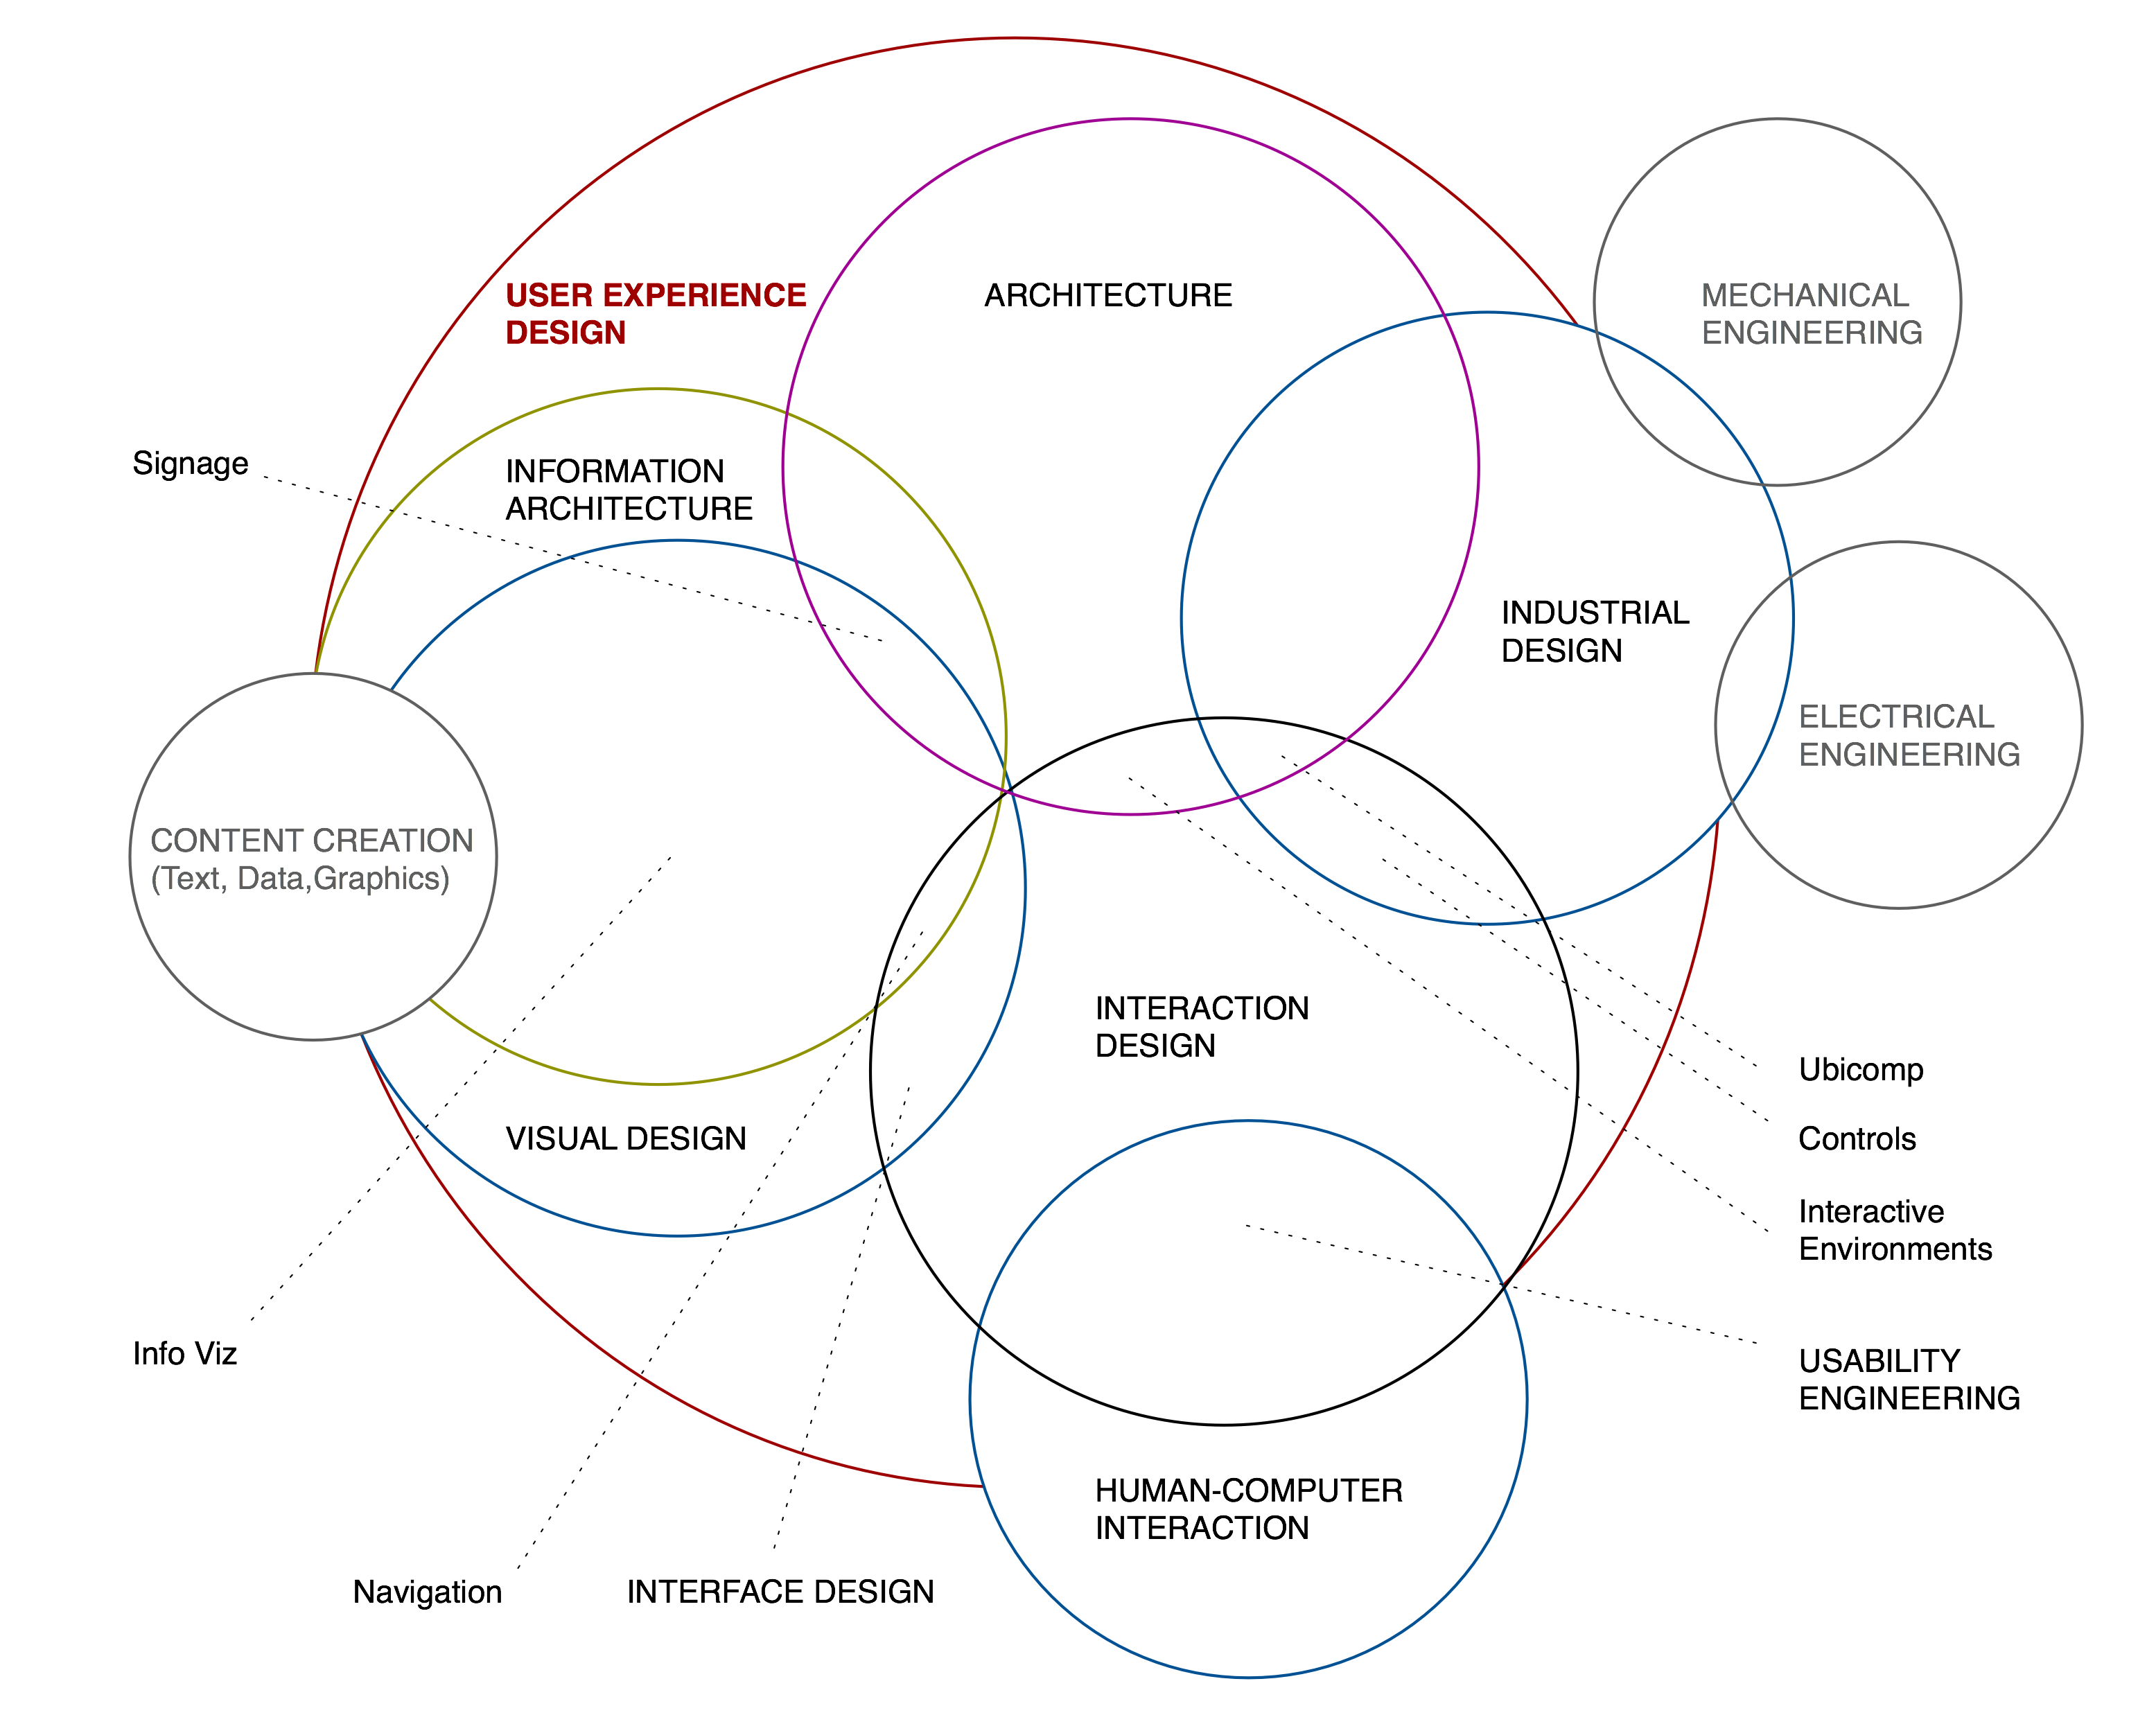
\includegraphics[scale=0.45]{ux.jpg}
  \caption{Saffers definition på UX\cite{SafferCreatingDevices}}
\end{figure} 

Norman säger att design kräver kunskap från flera områden vilket gör UX subjektivt och dess utvärderingsmetoder subjektiva \cite{NormanquotPeople}. Dillon menar att den upplevda användbarheten och dess tillfredsställande estetik är två kriterier som behövs ta hänsyn till för att förstå User Experience, medan andra forskare menar på att fokus bör vara på att arbeta med personen i sig \cite{Lee2010UnderstandingUse}. 

UX-området tar till hänsyn att värdesätta användarens upplevelse av en produkt eller tjänst vilket kan innebära att användaren gör ett ställningstagande runt dess estetik\cite{TuchIsHCI}. Det finns en växelverkan mellan hedonistiska faktorer och helhetsupplevelser av system \cite{TuchIsHCI}.
\newline


\subsubsection{Vår syn på User Experience}
Då User Experience har många definitioner har vi valt att tolka området på vårt sätt utifrån den fakta som samlats in. Enligt Bargas \cite{Bargas-AvilaOldExperience} är User Experience den personligt upplevda känslan kring en produkt eller tjänst, vilket också är sättet vi har tolkat UX på. Då det är viktigt att användaren kan interagera med en produkt eller tjänst på ett så enkelt sätt som möjligt så är en av grundprinciperna att sätta användaren i fokus. Detta är något vi samtycker med då många företag tenderar att implementera tjänster utefter deras behov istället för användaren \cite{PlaneradBokhandel}. Detta leder till funktionaliteter som inte uppnår användaren behov och tjänsten/produkten riskerar att inte bli nyttjad.
\newline

Det är viktigt med en tydlig distinktion mellan användbarhet och User Experience. De har mycket gemensamt, men UX tar till hänsyn att värdesätta användarens upplevelse av produkten och dess vilja att nyttja den. Detta kan innebära att användaren tar ett ställningstagande runt dess estetiska tilltalet, det vill säga om den är väldesignad och om användaren upplever att den är hedonistiskt tillfredsställande. Det finns samband där en god användbarhet har influerad testpersonens åsikt om den upplevda estetiken\cite{Gualtieri2009BestDesign}. Forskning visar på att en växelverkan mellan hedonistiska faktorer och helhetsupplevelser av system existerar\cite{TuchIsHCI}. Det är viktigt att icke-funktionella inslag av en produkt tas till hänsyn, där man gör en distinktion mellan användbarhet och UX. 
\newline

\subsection{Prototyper}
Att få en design perfekt vid första försöket är omöjligt vilket är allmänt känt för yrkesverksamma inom UX. Därför används prototyper i ett tidigt skede då man vill utvärdera design och funktionalitet \cite{Yamakami2014ExploratoryDesign}. För att få en god användarupplevelse behövs det utformas en testmodell. I kontext till denna studien är testmodellen en prototyp. I dess tidigaste skede, innan utveckling av kod görs, börjas det med skisser eller low-fidelityprototyper \cite{Gualtieri2009BestDesign}. Gualtieri\cite{Gualtieri2009BestDesign} förespråkar att utforma (designa) ett koncept i ett tidigt skede och använda sina slutanvändare för att utveckla designen vidare (läs mer om detta i sektion 2.6 Användartestning och utvärdering). Vad en prototyp är kan skilja sig oerhört, från att vara en välutvecklad interaktiv prototyp till en skiss på ett papper\cite{HoudeWhatPrototype}. Grundreceptet är att det går att testa och validera på slutanvändaren för att förstå hur det ska gås vidare i design och utvecklingsprocess\cite{HoudeWhatPrototype}.
\newline

Enligt Houde och Hill \cite{HoudeWhatPrototype} är en prototyp något som är till för att utforska och visa en design. De menar att det är en vedertagen metod att bygga en prototyp för att representera något i de olika stadierna av designen, och för att utforska möjligheter. Emellertid är interaktiva system komplexa där det kan vara svårt att skapa prototyper av en hel design \cite{HoudeWhatPrototype}.
\newline

Modellen i figur 2 är en bild som ska representera de viktigaste aspekterna i en design av en interaktiv prototyp. Bilden representerar Houde och Hill:s syn på vad en prototyp är och de menar på att de tre aspekterna som man bör ha i åtanke är\cite{HoudeWhatPrototype}:
\begin{itemize}
\item Rollen
\item Hur den ser ut och känns
\item Implementationen
\end{itemize}
Med \enquote{rollen} syftar de till frågor om funktionaliteten som har med användaren att göra. 
\enquote{Hur den ser ut och känn} har att göra med den konkreta upplevelsen om användarens estetiska intryck och hur användaren anser att den känns. Med \enquote{implementation} syftar Houde och Hill till frågor angående tekniken och de som kallar för UI (User Interface). Triangeln är gjord för att enkelt kunna visa vilka aspekter som är viktiga samt att ingen del är mer essentiell än den andra. Målet med modellen är att vid ett designproblem (oberoende av storlek eller dess omfång) ska triangeln behandlas som ett hjälpmedel för att separera diverse problem in i dessa tre klasser. Detta för att förstå de frågor varje klass sekventiellt ställs inför.

\begin{figure}[H]
  \centering
  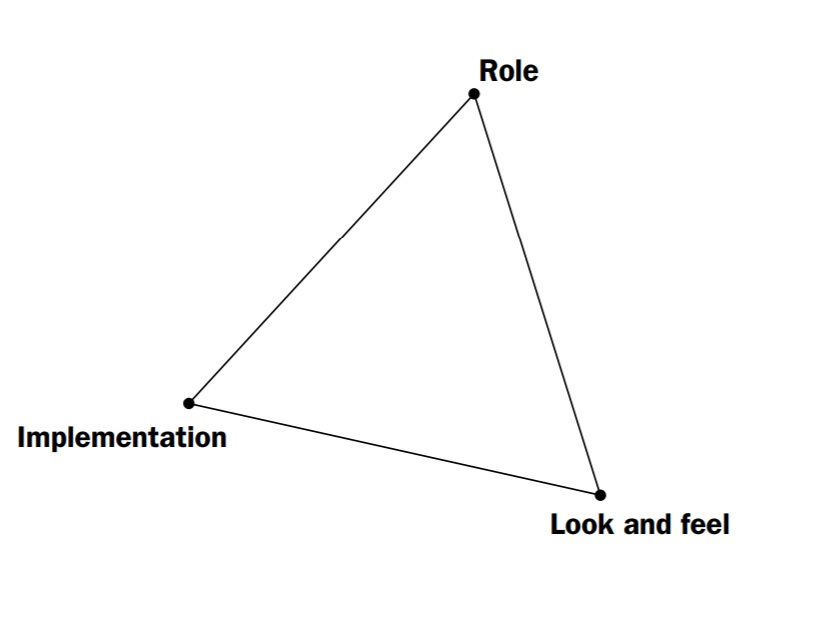
\includegraphics[scale=0.9]{resources/Prototyp.jpg}
  \centering
  \captionsetup{justification=centering, margin=2cm}
  \caption{Figur från \textit{What do Prototypes Prototype?} av Stephanie Houde och Charles Hill
 \cite{HoudeWhatPrototype} }
\end{figure}

Genom att explicit fokusera på vissa designfrågor kan man förstå vilken typ av prototyp som ska implementeras, hur den ska testas och vilken modell som hjälper att visualisera det fokus som ska vara efter utformning av syftet med applikationen\cite{HoudeWhatPrototype}. Således är de frågor man ska ställa sig, enligt Houde och Hill\cite{HoudeWhatPrototype}: 
\begin{itemize}
\item Vilken roll kommer det att spela i användarens liv?
\item Hur ska det se ut och känna? 
\item Hur bör det genomföras?
\end{itemize}

 Figur 2 och dess attribut är ett verktyg som kan användas för att prototypen ska uppfylla de syfte man vill att den ska göra -där olika prototyper har olika indelningar i de tre klasserna och svar på de frågorna ger en specifik fördel vid utformandet av den \cite{HoudeWhatPrototype}.


\subsection{Användartestning och utvärdering}
En mängd olika metoder har utvecklats för att stödja människocentrerad och användarcentrerad design\cite{Abras2004User-CenteredDesign}. Dessa metoder är bland annat användartester, heuristisk utvärdering, diskussionsutvärdering och deltagande design. 
\newline

Användartestning är en central del inom UX som betyder att man sätter slutanvändaren i centrum. Detta för att kunna undersöka om prototypen eller produkten når upp till kriterierna för god användbarhet och användarupplevelse för slutanvändaren\cite{Gualtieri2009BestDesign}.  En riktlinje som Gualiteri går in på är att man inte ska lita på någon, utan testa allt, där testresultat kan ge konkreta värden och väsentlig riktning av ett projekt\cite{Gualtieri2009BestDesign}.  
\newline
 
När en digital plattform formas behövs det utföras användartestning för att nå förväntningarna som en användare har på produkten. Gualtieri \cite{Gualtieri2009BestDesign} menar att det behövs göras vid ett tidigt skede när utformning av en produkt eller tjänst görs, så att man kan förstå användaren. Han menar också att användartestning ger resultat som kan ge riktlinjer som är essentiell vid utformningen av applikationen. Han nämner också att man lätt förväxlar kunden och slutanvändaren, då dessa nödvändigtvis inte delar samma behov eller mål. För att kunna utföra användartester krävs det att det finns något att testa på så som en modell, prototyp eller del av en applikation\cite{Gualtieri2009BestDesign}. Vredenbrug \cite{Vredenburg2002APractice} gjorde en fallstudie där han kom fram till att en iterativ design är en grundpelare för att få en användarcentrerad utveckling. 
\newline

Ett problem, som är viktigt att ha i åtanke vid utformning av ett användartest, är att den del/modell eller prototyp som testas på användaren bör vara väl fungerande där funktionaliteten inte ska vara begränsad till den utsträckning att det påverkar det estetiska tilltalet{\cite{Gualtieri2009BestDesign}. Det är viktigt att icke-funktionella inslag av en produkt tas till hänsyn vid användartester, där man gör en distinktion mellan användbarhet och användarupplevelse. Det är därmed viktigt att vara tydlig med syftet av användartestningen, så att man inte har fokus på funktionalitet utan fokus är på helhetsbilden av användarupplevelsen.
\newline

Enligt Benyon \cite{Benyon2013Designing3/E} är det viktigt att förstå att en undersökning i form av intervju eller enkät inte är tillräcklig, utan detta ska ske i kombination med observation för ett korrekt resultat. Testpersonen ska representera slutanvändaren, vilket betyder att hen nödvändigtvis behöver vara just den exakta slutanvändaren utan behöver tänka som slutanvändaren \cite{Benyon2013Designing3/E}.
\newline

\subsection{Kategorisering}
\label{kategorisering}
Människocentrerad design och användarcentrerad design är två ramverk som kan användas i varje vid utformning av produkt eller tjänst. Genom att använda ett UX-ramverk kan man på ett strukturerat sätt ta in alla dess olika attribut. Då UX definieras på många olika sätt så kan det vara en trygghet att luta sig mot ett studerat och testat ramverk. 
\newline

Konstruktionen av frågeformuläret samt frågorna till fokusgrupperna baseras Laugwitz, Held, och Schrepp's artikel "Construction and Evaluation of a User Experience
Questionnaire" \cite{Laugwitz2008ConstructionQuestionnaire}. Dem i sin tur utgick efter ett teoretiskt ramverk inom User Experience \cite{HassenzahlUserQuality}. Ramverket är framtaget av Hassenzahl och syftar till att gruppera två olika kvalitetsaspekter: ergonomisk kvalitet (EQ) och hedonisk kvalitet (HQ)\cite{HassenzahlUserQuality}. Ramverket särskiljer på upplevd ergonomisk kvalitet och upplevd hedonisk kvalitet. Detta används sedan för att kunna utvärdera hur attraktiv en produkt eller tjänst är, enligt Hassenzahl. 
\newline

Uppkomsten av Hassenzahls ramverk grundar sig på begreppet användbarhet, inom Människa- datorinteraktion, där han menar att användbarhet inte tillgodoser faktorer om huruvida produkten eller tjänsten är rolig att använda \cite{HassenzahlUserQuality}. Han menar också att användbarhet inte tar hänsyn till preferenser vad det gäller användarens tillfredsställelse. Därför föreslogs en ny modell som inkluderade "hedonisk kvalité" \cite{HassenzahlUserQuality} . 
\newline

Ergonomisk- och hedonisk kvalitet är två kategorier som sammanfattar olika kvalitetsaspekter\cite{HassenzahlUserQuality}. Ergonomisk kvalitet innebär att man ser till den målorienterade eller arbetsorienterade aspekterna i designen av en produkt eller tjänst\cite{HassenzahlUserQuality}. En hög ergonomisk kvalitet innebär att användaren kan nå uppgiftsorienterade mål på ett effektivt sätt\cite{HassenzahlUserQuality}. Hedonisk kvalitet syftar till vad användaren tycker om produktens estetik eller attraktivitet\cite{HassenzahlUserQuality}. Här är aspekter som uppgiftsorienterade mål, jämfört med ergonomisk kvalitet, inte viktigt\cite{HassenzahlUserQuality}. 
\newline

Personer antas således uppfatta flera olika aspekter vid en utvärdering av en produkt\cite{HassenzahlUserQuality}. Kontrapunkten mellan ergonomisk och hedonisk kvalitet bör således tas till hänsyn vid en undersökning av en produkt\cite{Laugwitz2008ConstructionQuestionnaire}. Enligt detta antagande bör frågeformuläret innehålla två indelningar enligt Laugwitz, Held, och Schrepp\cite{Laugwitz2008ConstructionQuestionnaire}:
\begin{itemize}
\item den uppfattade attraktiviteten (EQ) och
\item den uppfattade kvaliteten på relevanta aspekter (HQ).
\end{itemize}

Frågeformuläret som utformades av Laugwitz, Held, och Schrepp arbetades fram med hänsyn till UX-ramverket av Hassezahl \cite{Laugwitz2008ConstructionQuestionnaire}. De arbetade iterativt fram olika kategorier som tog hänsyn till EQ och HQ. Kategorierna omfattade de två indelningarna vid undersökning av en produkt: den uppfattade attraktiviteten och den uppfattade kvaliteten på relevanta aspekter. Tillslut kom de fram till fem kategorier\cite{Laugwitz2008ConstructionQuestionnaire}: 
\begin{itemize}
\item Tydlighet
\item Effektivitet
\item Pålitlighet
\item Stimuli
\item Attraktivitet
\end{itemize}

Dessa kategorier har vi använt som grund till vår analys och utvärdering på AL1 prototypen. 

\subsubsection{Anledning till val av att använda kategoriseringen}

Olika applikationer har mer eller mindre krav beroende på syftet med användandet av applikationen\cite{UXUX}. Dessa krav berör också upplevelsen som användaren har. Ett exempel på detta är en applikation som har att göra med transaktioner, betalningsmetoder eller pengar att göra.I en sådan applikation har användaren höga krav på tydlighet så att funktionaliteten flyter på\cite{UXUX}. Användaren behöver i detta fall uppleva att applikationen är pålitlig, där utseendet (attraktiviteten) inte är ett högt krav\cite{UXUX}. Som Hassenzahl menar, när en användare gör en utvärdering av en applikation så vägs olika egenskaper in vid bedömningen. Forskare inom designteknik, exempelvis Karat, Lindgaard och Bassat\cite{Ben-BassatEconomicUsability}\cite{LindgaardWhatSatisfaction} \cite{Karat2003TheField}, indikerar på att designtekniken har en inverkan på preferenser hos användaren. Således behöver man behärska både syftet med applikationen och vad slutanvändaren anser vara viktigast för användarupplevelsen. Om man vill att applikationen ska vara användarcentrerad behöver man förstå vilken aspekt som är viktigast och göra en prioritering \cite{5Foundation}.
\newline

Det är anledningarna till varför vi valt att arbeta med de kategorier som utformats av Laugwitz, Held, och Schrepp  för att undersöka vad användaren tycker om Amazing Leaders prototyp. 







\newpage
\section{Uppdragsgivare och resurser}
I det här kapitlet går vi in djupare på
vilka uppdragsgivarna är, samt den prototyp vi har tagit del av. Kapitlet ska ge dig som läsare en bakgrund för att förstå rapporten bättre.  

\subsection{VNTRS}
VNTS är ett konsultbolag som har sin bas i Stockholm. VNTRS grundades av fyra managementkonsulter. Deras vision är att hjälpa entreprenörer samt stora företag med innovativa digitala produkter och tjänster. VNTRS har i nuläget, Maj 2018, 21 anställda i sitt bolag. De har junior samt seniora konsulter som har erfarenhet inom iOS-utveckling, Android-utveckling, Frontend-utveckling, Backend- och UX / UI-utveckling tillsammans med personer som arbetar med marknadsstrategi. De hjälper sina kunder att utveckla en del i eller en hel digitala produkt eller tjänst, beroende på behov och uppdrag. VNTRS har utvecklat digitala produkter så som Byt Grej, Zipo, SUNI och BakingHood\cite{VNTRSAB}och har arbetat med bolag som Office Depot, NRK och Husbanken. 

\subsection{Amazing Leaders}
I den här studien är vår uppdragsgivare Amazing Leaders, där deras jobb går ut på att möjliggöra framgångsrikt ledarskap med hjälp av individers emotionella talang. De jobbar med kunder som exempelvis Telia, SEB och Adidas där de arbetar tillsammans med kund för att engagera och få en ledareffektivitet. Termen EQ-smart är något de lyfter fram där de tillsammans med diverse program vill öka individers emotionella intelligens. Emotionell intelligens kan handla om ens förmåga att kunna känna igen och kontrollera känslor hos en själv och andra. Amazing Leaders EQ ramverk är baserat på psykologen Martyn Newmans definition och forskning om EQ. Detta ramverk skapade en röd tråd inom Amazing Leaders där de arbetar med att utveckla människors och verksamheters emotionella intelligens, för att nå hållbara resultat. 
\newline

De menar på att för att få ett högpresterande team och en ledareffektivitet behöver man jobba på EQ. De har tjänster som individuell coachning, teamutveckling, ledarskapsprogram, karriärcoachning för att nämna några. De åstadkommer att utbilda individer om EQ genom digiloga processer, där man har mänskliga möten med digitalt stöd. Genom att jobba med EQ har de kunnat jobba med den forskningen som fanns vilket har möjliggjort att mäta resultat kopplat till deras kunders KPI:er (Keep Performance Index). Idag har deras rapporter och resultat visat på att emotionellt starka människor är bättre ledare som i sin tur skapar effektivare och konkurrenskraftigare företag. {\cite{AmazingLeaders2017OmLeaders}}
\newline

\subsection{AL1 - prototypen}
Den prototyp som använts i denna studie har utformats av VNTRS. AL1 innehåller i sin helhet en video på en av Amazing Leaders' coacher, Ursula. Syftet med prototypen var att få en inblick i hur den framtida applikationen skulle komma att se ut. Prototypen börjar med att Ursula pratar informativt om värderingar. Sedan får användaren stegvis svara på olika frågor under videons gång. Användaren får svara på frågor genom att klicka i förvalda alternativ på en skala samt genom att själv få skriva i sina svar. I slutet visas en graf som ska representera dina värderingar baserat på vad du som användare har svarat.
\newline

\begin{figure} [H] 
  \centering
  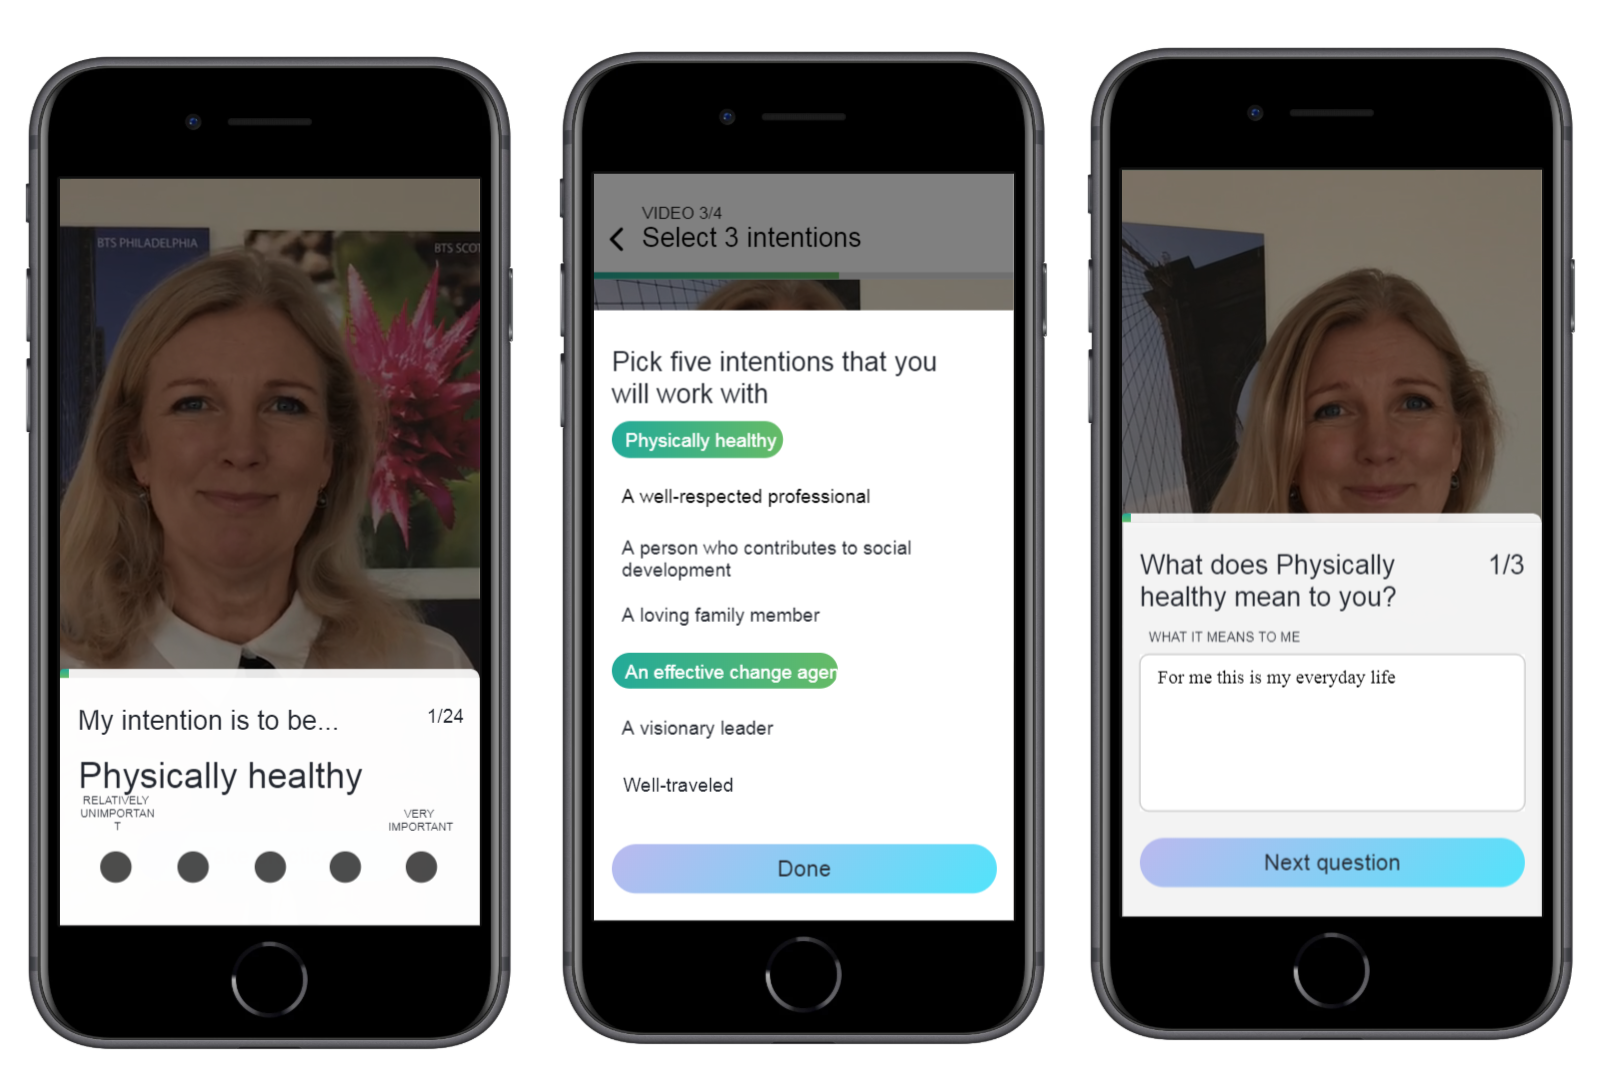
\includegraphics[scale=0.3]{AL1.png}
\centering
\captionsetup{justification=centering,margin=2cm}
\caption{Bild på AL1 som visar olika svarsalternativ}
\end{figure} 
Prototypen har som tydligt mål att användas i syfte av att testa användarupplevelsen, det vill säga den övergripande interaktionen som testperson har med prototypen. Besläktade testområden som användbarheten utesluts från prototypens ändamål. Eftersom att det fanns en risk att prototypen hade brister, utbildades testpersoner kort om distinktionerna mellan användbarhet och användarupplevelse. 
\newline




\newpage
\section{Metod}
I den här delen av uppsatsen presenteras metodvalen som är relevanta för studien och anledning till varför dem valdes. För att få en bred uppfattning om användarens uppfattning av AL1 genomfördes denna studie enligt triangulering: \textit{litteraturstudie, fokusgrupper} och \textit{enkätundersökningar}. 

\subsection{Tillvägagångssätt}
\label{sec:background}
Studien hade som syfte att utforska den totala användarupplevelsen av AL1-prototypen. Det var viktigt att metodvalet var tydligt och konkret, där uppsättningen av krav för studien bemöttes och där aspekter från litteratur och forskningsområdet togs i åtanke. 
\newline

Studien använde metoden triangulering för att öka validiteten och har bestått av \textit{litteraturstudie, fokusgrupper och enkätundersökningar} \cite{RankinKvalitativaMetoder}. En litteraturstudie gjordes för att få en teoretisk bakgrund som krävdes för projektet samt för att kunna välja relevant utvärderingsmetoder. Det som var mest relevant för studien efter att ha analyserat teorier vid liknande studier var Hassenzahls ramverk \cite{HassenzahlUserQuality} samt Lauqwitz et al. kategorisering\cite{Laugwitz2008ConstructionQuestionnaire} (läs mer om ramverket och kategoriseringen under Kategorisering i sektion \ref{kategorisering}). Efter utformningen av enkätundersökningen upptäcktes det att ett komplement behövdes för att täcka frågeställningarna. Något som togs i åtanke under studiens gång var konceptet \enquote{gap-filling}. Det är en ansats som Alvesson och Sandberg \cite{Alvesson1985GENERATINGPROBLEMATIZATION} menar är när en undersökning är otillräcklig eller icke övertygande. Detta ger i sin tur upphov till obesvarade frågor eftersom att det funnits ett spektrum som inte problematiserats eller ifrågasatts. 
\newline

I studien användes två utvärderingsmetoder; enkätundersökningarna och användartest i form av fokusgrupper. Dessa metoder genomfördes sedan på slutanvändaren(målgruppen). Resonemanget till varför fokusgrupper och enkätundersökning valdes var för att få möjligheten att behandla kvantitativ data tillsammans med en kompletterande kvalitativ data. Det valdes att arbeta på ett abduktivt arbetssätt, det vill säga att vi systematiskt arbetat med en kombination av hypoteser och blandat dem med observation. 

Abduktion rymmer kunskapsfilosofiska teorier om människan, verkligheten och relationen dem emellan, men är också en forskningsmetod som bygger på att upptäcka det oväntade, stämma av det mot befintlig kunskap, skapa ny förståelse som sedan prövas genom nya iakttagelser i en levande och ständigt pågående process. \cite{Langendoen1999HowWorks}

En stor del av arbetet har varit att dra slutsatser från givna premisser, vilket är anledningen till ett akduktivt arbetssätt. Det är en av anledningarna till det valda ramverket skapat av Hassenzahl \cite{HassenzahlUserQuality} och varför kategoriseringen är central. 
\newline

\subsection{Litteraturstudie}
Vid studiens start gjordes en grundlig litteratur studie för att få nödvändig information om användbarhet och UX. Relevant litteratur togs fram i form av böcker och artiklar. I ett tidigt skede utforskades främst erkända böcker inom området, så som: 
\textit{Designing Interactive Systems by Benyon (2010)} och \textit{The design of everyday things by Norman (2002)} studerade. Den här ordningen var fundamental för att få rätt information om området. Kunskap om UX området togs fram genom grundlig studering av relevanta artiklar som exempelvis \textit{Gualiteri Best Practices In User Experience (UX) Design (2001)} och \textit{The Effect of Perceived Hedonic Quality on Product Appealingness av Marc Hassenzahl(2001)}. 
\newline

Syftet med litteraturstudien var också att finna specifik information som var nödvändig för att genomföra studien. Ett antal databaser användes för att hitta artiklar och journaler; ACM, Google Scholar, DIVA portalen och IEEE. Processen gick ut på att söka på nyckelord som kunde ge väsentliga artiklar. De nyckelord som användes vid sökningen var bland annat; \textit{Human Computer Interaction ,  Usability, User Experience,UX, HCI + Usability + User Experience, UX + Questionnaire.} 
\newline

Tillvägagångssättet som användes vid analys av källkritik på källorna genomfördes med hjälp av skolverkets riktlinjer\cite{GuideKallkritik}. Dessa riktlinjer avser att undersöka källans äkthet. De punkter som togs i åtanke vid den källkritiska analysen var\cite{GuideKallkritik}: 
\begin{itemize}
\item Finns något syfte med publiceringen?
\item Är informationen trovärdig?
\item Stämmer det med vad du redan vet?
\item Hittar du något budskap?
\item Finns dolda budskap?
\item Går fakta att kontrollera?
\item Saknas uppgifter?
\end{itemize}
Dessutom gjordes en jämförelse mellan olika källor som behandlade samma ämne, för att undersöka källans äkthet och så att det inte låg personliga budskap eller att informationen var vinklad på något sätt. Sökningen avslutades då tillräckligt med relevant information blev framtaget för att göra och forma utvärderingsmetoderna. 

\subsection{Enkätundersökning}
Enkätundersökningar är en enkel och vanlig metod för att få snabba svar samt för att få hjälpsam feedback om hur interaktionen med produkten är och hur det känns att använda den. Rent praktiskt kan det anses vara väldigt enkelt att genomföra, det är bara att skicka till ett urval av personer och man får snabba svar\cite{Paloma201499Paloma}. Däremot är det inte lika enkelt att få svar som verkligen kommer att ge värdefull feedback på en prototyp. Sådana frågeställningar kräver planering, eftertanke och noggrannhet\cite{KundKoll2018TipsKundkoll}.
\newline

Ett tydligt mål av undersökningen behövs därför vid utformningen av enkäten, hur kommunikationen ska ske, de åtgärder som kommer att göras från resultatet och uppföljningen. Frågor behöver vara ställda på ett sådant sätt att alla respondenter uppfattar dem på samma sätt vilket gör att hur enkelt det är att förstå frågan är en viktig faktor. Med en tydlig och väl utformad enkät menas därför att ge rätt och välformulerade svarsalternativ så det inte uppfattas olika beroende på respondent. En nyckel till detta är att göra olika varianter på samma fråga och testa, samt upprepa samma fråga med olika ord för att säkerställa att datan man får in är korrekt. Tydligheten påverkar också tiden som behövs läggas på en enkät där man vill hålla det så kort som möjligt för ökad deltagande, detta då respondenterna kan ha begränsad tillgång på tid \cite{Vannette20154Qualtrics}. Användaren ska dessutom kunna ge sin bedömning av produkten utan att behöva gå tillbaka och granska den igen, syftet är alltså att undvika en djupare analys vid en enkätundersökning \cite{Laugwitz2008ConstructionQuestionnaire}. 
\newline

En stor fördel med enkätundersökningar är att det kan nås ut till ett stort urval av människor då det är enkelt att skicka ut undersökningen digitalt via webben \cite{Boynton2004SelectingQuestionnaire}. Respondenterna kan också sitta i lugn och ro och svara på undersökningen vilket ger upphov till en bredare grad av reflektion innan man svarar på frågorna \cite{Boynton2004SelectingQuestionnaire}. Däremot är en klar nackdel att respondenten inte kan ställa frågor om något skulle vara oklart vilket gör att man kan misstolka en eller flera frågor. Detta kan också leda till ett visst bortfall av respondenter på grund av deras begränsade tid, vilket är beroende av tydligheten på frågorna \cite{Boynton2004SelectingQuestionnaire}. 


\subsection{Fokusgrupper}
För att angripa problemet från flera synvinklar och dessutom fördjupa resultatet från enkätundersökningen har vi valt att samla in kvalitativ data genom fokusgrupper, vilket är en systematiserad gruppintervju \cite{FokusgruppGruppintervju}. Syftet med fokusgrupper har varit att få fram användarupplevelsen i sin helhet. Vid användandet av fokusgrupper får man inte bara data om vad en grupp individer tycker och tänker, utan även information om varför. 
\newline

Den stora fördelen med fokusgrupper är att det sker en interaktion emellan deltagarna själva. Vid en intervju står intervjuaren i centrum och interaktionen är mellan intervjuare och respondent, jämfört med en fokusgrupp där deltagarna uppmuntras att dela med sig av sina synpunkter samt att lyssna på de andra deltagarna och ett av målen är att ha en givande diskussion. Morgan menar att fokusgruppers interaktion mellan deltagarna själva är lika mycket en fallgrop som styrka\cite{MorganFocusGroups}. Det som kan ske är att några deltagare dominerar diskussionen och därför är det viktigt att samtalsledaren är aktiv genom att låta alla komma till tals och styra diskussionen så den faller inom forskningsområdet och håller en röd tråd \cite{TuckmanModel}. Det finns studier som visar att fokusgrupper bör ha en samtalsledare i undersökningen, där en agerar som moderator och en som observatör \cite{Denscombe2010TheProjects}. 
\newline

Fokusgrupper är en lämplig utvärderingsmetod när man vill ha en förståelse för hur slutanvändaren resonerar eller upplever runt ett visst ämne \cite{MorganFocusGroups}. Fokusgruppens deltagare kan antingen enas, vilket kan resulteras i ett överenskommande. Alternativt så kan uppfattningen skilja sig åt, som resulterar i att det kan finnas en komplexitet runt AL1 eller enskilda delar av AL1. Vid en diskussion sker ett utbyte av åsikter där man kontinuerligt förhandlar och resonerar runt sitt ställningstagande. Vi vill i vår studie lyfta denna interaktion då den är central i vår forskningsfråga, där det kan bidra till en förbättrad slutprodukt\cite{VictoriaWibeck2010FokusgrupperUndersokningsmetod}.Genom att undersöka interaktionen mellan deltagarna och i den bemärkelsen observera och konstatera utmaningar, nöjdhetsfaktorer eller problem så kan resultat tas fram som i sin tur möjliggör att förbättringar kan ske. 


\newpage
\section{Utförande - (working title)}
I det här kapitlet beskrivs det praktiska tillvägagångssättet mellan metod och resultat. Först presenteras utformningen av enkät, och dess undersökning följt av genomförandes av denna.
Fokusgrupperna beskrivs analogt. 
\subsection{Utformning av enkätundersökning}
När enkätundersökningen utformades hade vi Laugwitz, Held, och Schrepp's arbete \enquote{Construction and Evaluation of a User Experience
Questionnaire} som riktlinje och mall\cite{Laugwitz2008ConstructionQuestionnaire}. Deras mall användes eftersom att ramverket föddes ur en djup forskning inom området UX, och var avsedd för applikationer så som våran, det vill säga extraheringen av information från en befintlig produkt/prototyp. Användarupplevelsen delas upp i delar vilket Laugwitz et al. kallar för kategorisering (se mer om detta under sektionen Kategorisering \ref{kategorisering})\cite{Laugwitz2008ConstructionQuestionnaire}.\\

Boynton och Greenhalgh menar på att en nyckelpunkt när man utformar ett frågeformulär är att använda tidigare validerade formulär\cite{Boynton2004SelectingQuestionnaire}. Således var utgångspunkt mallen \enquote{Construction and Evaluation of a User Experience
Questionnaire} och sedan formades en enkät med frågor för att få svar på det som besvarar studiens forskningsfråga och är i studiens omfång.  

\subsubsection{Kategorisering}
Eftersom att frågor ofta är vinklade kan man ställa samma fråga fast på olika sätt för att få ett mer exakt svar. Det var på detta sätt som frågorna arbetades fram enligt Laugwitz et al. \cite{Laugwitz2008ConstructionQuestionnaire}. Kategoriseringen som skall täcka hela användarupplevelsen enligt Laugwitz et. al \cite{Laugwitz2008ConstructionQuestionnaire} gör att man kan ta fram en skala för empirisk data. Skalan är från 1 till 6 där respondenten kan välja ett alternativ på varje fråga. Varje kategori hade liknande frågor som ställdes på olika sätt för att säkerställa respondentens svar och sen kunna ta fram en total bedömning på den användarupplevelsen av AL1 (se hela enkäten i Bilaga B). Läs mer om detta under sektionen Kategorisering \ref{kategorisering}.
\newline

Frågorna som ställdes i enkätundersökningen var: 

\begin{enumerate}
\item \textbf{Attraktivitet:}
\newline
Jag upplever att prototypens totala intryck är:
\begin{itemize}
\item Ful/Snygg
\item Irriterande/Angenäm
\item Otrevlig/Tilltalande
\newline
\end{itemize}

\item \textbf{Effektivitet:}
\newline
Mitt totala intryck av prototypen är att den går/är:
\begin{itemize}
\item Långsam att använda/Snabb att använda
\item Ineffektiv/Effektiv
\item Opraktisk/Praktisk
\item Rörig/Välorganiserad
\newline
\end{itemize}


\item \textbf{Pålitlighet:}
\newline
Jag upplever prototypen som:
\begin{itemize}
\item Oförutsägbar/Pålitlig
\item Komplicerad/Enkel
\item Förvirrande/Tydliga instruktioner
\newline
\end{itemize}


\item \textbf{Tydlighet:}
\newline
Jag upplever prototypen som
\begin{itemize}
\item Svår att förstå/Lätt att förstå
\item Hämmande/Underlättande
\item Oviktig/Viktig
\newline
\end{itemize}

\item \textbf{Effektivitet:}
\newline
Jag upplever prototypen som
\begin{itemize}
\item Omodern/Modern
\item Oinspirerande/Inspirerande
\item Jobbig/Bekväm
\newline
\end{itemize}

\end{enumerate}

I bilaga B kan det fullständiga frågeformuläret hittas. 

\subsection{Genomförande av enkätundersökning}
Enkäten skapades i Google Forms \cite{GoogleForms}, detta för att det är ett enkelt system för utformning av en enkät och dessutom väldigt enkelt att sprida, med hjälp av en länk. När utkastet till enkäten var färdigställd så testades den på ett antal utomstående personer där de fick gå igenom prototypen och svara på enkäten. Vid testningen av enkäten klarades frågetecken ut och revidering efter kritik verkställdes. Denna feedback var viktig för att försäkras om att frågorna var ställda på ett sådant sätt att betraktaren skulle förstå varje fråga och för att datan som samlades in inte skiljde sig mellan respondenterna. 
\newline

Enkäten skickades ut till relevanta personer, via Linkedin och e-mail. I beskrivningen presenterades vilka vi var och syftet med enkäten. Enkätundersökningen genomfördes digitalt tillsammans med prototypen och tillhörande frågor om den. 
\newline

\subsubsection{Målgrupp (Urval)}
Målgruppen för respondenter har varit framtida slutanvändare till applikationen. När urvalet av personer som skulle få möjligheten att svara på enkätundersökningen gjordes resonerades det fram till att personer inom en organisation som vill lära sig mer om EQ var de som var lämpliga att svara på enkäten. 
\newline

Urvalet har utgått från Amazing Leaders' kontakter och sedan varit ett snöbollsurval\cite{RankinKvalitativaMetoder}. Snöbollsurval är ett icke-slumpmässigt urval av personer som man med hjälp av tidigare valda personer letar sig fram till andra personer som man kan ha med i urvalet. \cite{VejdeSnobollsurval} Detta var lämpligt då Amazing Leaders har haft ett brett nätverk där de i sin tur vetat andra som passar målgruppen. Enkäten skickades ut till sammanlagt 60 personer.
\label{sec:perspektiv}


\subsection{Utformning av fokusgrupp}
%När man utformar en fokusgrupp ska man vara medveten om vissa aspekter som: 
%\begin{itemize}
%\item Problemformuleringen 
%\item Målgruppen (urval) 
%\item Genomförande 
%\item Analysarbetet
%\end{itemize}
%\subsubsection{Problemformulering}
När man utformar en fokusgrupp vill man i sin bredaste grad få svar på hur användaren upplever prototypen, vilket har varit utgångspunkten av vår studie. Vi vill få fram utmaningar, helhetsupplevelsen och spekulera kring framtida förbättringar. För denna typ av studie resonerade det sig i att utformningen bör ha en samtalsledare och därför lämpar sig semi-strukturerade och ostrukturerade intervjuer bäst \cite{Denscombe2010TheProjects}. En semi-strukturerad intervju innebär att frågor skrivs som ett bedömningsunderlag där man under intervjuns gång kan fråga relevanta följ frågor, vilket lämpade sig för det skapade känslan av ett samtal vilket ökar  diskussionen \cite{RankinKvalitativaMetoder}. Att jobba med en ostrukturerad intervjuteknik är att man utfår från ett blankt papper där respondenten får styra samtalet\cite{PaUtvarderingsmetodikExperience}. En växelverkan mellan dessa metodiker ansågs passa bäst då den ostrukturerade intervju-tekniken gör att forskaren kan vara moderator med syfte att ingripa så lite som möjligt under intervjun för att tillåta gruppen diskutera fritt. Genom att utföra enkätundersökningarna först får vi förutsättningar att upptäcka vilka områden inom UX som var \enquote{gap-filling} och i fokusgrupperna undersöka utövandet av UX med detta i åtanke, se mer om vad \enquote{gap-filling} innebär under Metod~\ref{sec:background} \cite{Alvesson1985GENERATINGPROBLEMATIZATION}. 
\newline

\subsubsection{Kategorisering}
Precis som enkätundersökningarna följer fokusgrupperna kategoriseringen av Laugwitz et al \cite{Laugwitz2008ConstructionQuestionnaire}. Studiens målsättning har varit att ha ett kvalitativt tillvägagångsätt för att komplettera enkätundersökningens resultat. Läs mer om detta under sektionen Kategorisering \ref{kategorisering}. 
\newline

Frågor som ställdes på tillfällena var: 
\newline
\begin{enumerate}
\item \textbf{Attraktivitet}
\begin{itemize}  
\item Vad tycker du om det allmänna utseendet av prototypen, är den inbjudande att använda rent utseendemässigt?
\item Varför?
\item Varför inte?
\item Vad var bra och varför? 
\item Vad var dåligt och varför?
\item Hur viktigt är det för din användarupplevelse? Rösta från 1/10 till 10/10, skriv ditt svar på denna lapp
\end{itemize}

\item \textbf{Tydlighet}
\begin{itemize}  
\item Hur tydlig är prototypen, är det lätt att förstå vad som förväntas av dig som användare? Är det lätt att förstå hur man tar sig till nästkommande steg?
\item Varför?
\item Varför inte?
\item Vad var bra och varför? 
\item Vad var dåligt och varför?
\item Hur viktigt är det för din användarupplevelse? Rösta från 1/10 till 10/10, skriv ditt svar på denna lapp
\end{itemize}

\item \textbf{Pålitlighet}
\begin{itemize}  
\item Hur pålitlig(känns den seriös/oseriös) känns prototypen? Känns den trovärdig? 
\item Varför?
\item Varför inte?
\item Vad var bra och varför? 
\item Vad var dåligt och varför?
\item Hur viktigt är det för din användarupplevelse? Rösta från 1/10 till 10/10, skriv ditt svar på denna lapp
\end{itemize}

\item \textbf{Stimuli}
\begin{itemize}  
\item Hur modern är den, är den “i tiden”? Känns den rolig/stimulerande att använda? 
\item Varför?
\item Varför inte?
\item Vad var bra och varför? 
\item Vad var dåligt och varför?
\item Hur viktigt är det för din användarupplevelse? Rösta från 1/10 till 10/10, skriv ditt svar på denna lapp
\end{itemize}

\item \textbf{Effektivitet}
\begin{itemize}  
\item Hur effektiv och snabb kändes den? Var den praktisk och organiserad? 
\item Varför?
\item Varför inte?
\item Vad var bra och varför? 
\item Vad var dåligt och varför?
\item Hur viktigt är det för din användarupplevelse? Rösta från 1/10 till 10/10, skriv ditt svar på denna lapp
\end{itemize}
\end{enumerate}

\subsection{Genomförande av fokusgrupp}
I samarbete med Amazing Leaders kom vi fram till att ha tre olika tillfällen i deras lokaler för att genomföra fokusgrupperna. För att generera en positiv ton och öka intresset hos deltagarna och för att säkerställa att deltagarna dök upp gjorde vi ett frukostevenemang, lunchevenemang och ett kvällsevenemang där vi bjöd på mat och dryck. Som tidigare diskuterat resonerade vi att mindre fokusgrupper skulle ge deltagarna mer utrymme för diskussion och ge möjlighet för alla att komma till tals. Grupperna formades efter våra kriterier, se sektionen Målgrupp nedan (5.4.1). Vi ansåg att en bra diskussion skulle kunna fortlöpa om deltagarna inte kände varandra eller jobbade på samma arbetsplats. Anledningen till bakom varför vi valde att forma grupperna på detta har att göra med att vi ville bibehålla alla deltagarnas relationsmässiga integritet. Vi ville inte att tidigare relationer och redan etablerade gruppdynamik skulle reflekteras i de svar som samlades in, och att deltagarna istället skulle få utrymma att tala fritt utan inverkan av extern påverkan. 
\newline


\subsubsection{Målgrupp (Urval)}
\label{malgrupp}
För att i en undersökning kunna dra slutsatser där data är validerad behöver man ta hänsyn till området, målgrupp\cite{Gualtieri2009BestDesign}. Vid möten med Amazing Leaders förstod vi att de hade ett stort urval av kontakter som skulle vara slutanvändaren. Då Amazing Leaders har en stor kundkrets behövdes det göras ett urval inför fokusgrupperna. Det urval som gjordes inför fokusgrupperna baserades på kriterierna: 
\begin{itemize}
\item Ålder
\item Bakgrund 
\item Yrkesverksamma år
\item Position i företaget 
\end{itemize}

Kartläggningen och ansatsen gjorde att vi fick ett diversifierat urval av erfarenhet, kön, anställning, bakgrund, utbildning, yrkesverksamma år och position i företaget. 

\subsection{Analys} 
För att kunna utvärdera den insamlade data, och avgöra vilka aspekter av användarupplevelsen som är viktigast, enligt respondenterna, presenteras insamlad data i stapeldiagram. Eftersom att datan som är insamlad är en indikation på hur viktig en kategori är för en bildar stapeldiagrammen bra översikt för hur fördelningen ser ut i gruppen som deltog i enkätundersökningen. Vidare kunde slutsatser om hur viktiga de olika kategorierna var för deltagarna i undersökningen dras. 
\\

För fokusgrupperna har vi använt oss av ljudinspelningar och anteckningar. Fokusgrupperna varade i en timme vardera där vi transkribera materialet på detaljnivå. Efter det började vi kategorisera och hitta gemensamma nyckelord och påståenden som var snarlika varandra. Vi anser att detta var ett viktigt stadium för att kunna strukturera upp och få fram data för vår forskningsfråga. Viktiga och meningsfulla diskussions ämnen redovisas som citat, där citaten tilldelas till relevant kategoriseringsämne. Se hela diskussionerna i Bilaga B.
\newline




\newpage
\section{Resultat}
I den här delen av rapporten kommer resultaten att presenteras. Resultatet redovisas kategorivis utefter Laugwitz et al. \cite{Laugwitz2008ConstructionQuestionnaire} bedömning av användarupplevelse, en riktlinje som använts i denna rapport, vilket är: 
\begin{itemize}
\item Tydlighet
\item Attraktivitet
\item Stimuli
\item Effektivitet
\item Pålitlighet
\end{itemize}
Resultat från både enkätundersökningar och fokusgrupper kommer att redovisas.
För mer information om kategorierna se avsnitt \ref{kategorisering}.\\

Av de 60 personer som enkäten skickades ut till fick vi 24 svar.  15 människor kunde samlas till fokusgrupperna med fem deltagare i vardera grupp under tre tillfällen. \\

% Sammanställningen av resultatet är i tre delar, där första delen är ett stapeldiagram på hur värdeskapande/viktigt kategorin är för slutanvändarens användarupplevelsen. Hur viktigt en specifik i varje kategori är blir representerat på en skala från 1-10 där en 10a är högsta betyg. Ju högre betyg det är för en kategori desto viktigare är den delen för användarupplevelsen. 
% \\

% Den andra delen är en bild som visar utvärderingen på AL1. Först visas medelvärdet som besvarar frågan, \textit{hur viktigt användarupplevelsen är}. Det följs av utvärderingen på prototypen som är en sammanställning på enkätfrågorna. Figuren representerar en total på de olika svarsalternativen 1-6 där en 6a är högsta betyg. Ju högre betyg det är för en kategori desto positivare har användarupplevelsen varit. 
% \\

% Sist kommer resultatet från fokusgrupperna. Vad fokusgrupperna diskuterade presenteras nedan grupperat efter kategori. Med utvalda citat för varje del.\\

% För hela diskussionerna av fokusgrupperna och enkätundersökningens frågor se bilaga A och B.
 
\subsection{Tydlighet}
Hur viktigt tydlighet är för användarupplevelsen är representerat från 1-10 där 10 är högsta betyg. Ju högre betyg det är för en kategorin desto viktigare är det för användarupplevelsen. Stapeldiagrammet presenteras i procentsatser för att ge en bättre översikt. 
\newline

\centerline{\textbf{Hur viktigt är tydlighet för 
din användarupplevelse}}
\begin{figure} [H] 
  \centering
  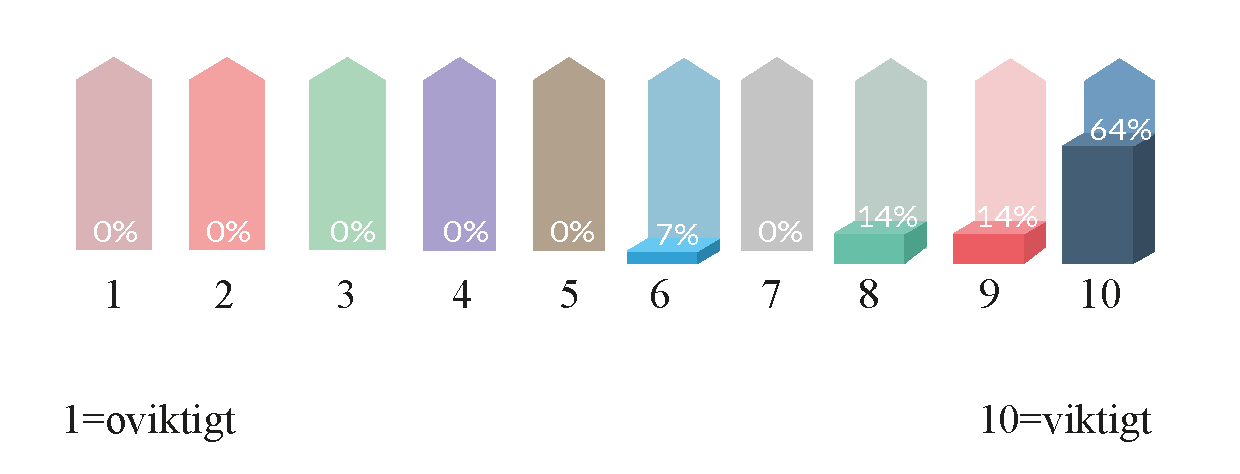
\includegraphics[scale=0.7]{Rityta_10.pdf}
\centering
\captionsetup{justification=centering,margin=2cm}
\caption{Resultat i procentuell skala på respondenternas svar}
\end{figure} 

Medelvärdet av ovan figur är 9.29. Siffran representerar ett medelsnitt av stapeldiagrammet som visar hur viktigt det var för användarupplevelsen enligt kategoriseringen framtagen av Hazzendahl. 


\begin{figure} [H]
  \centering
  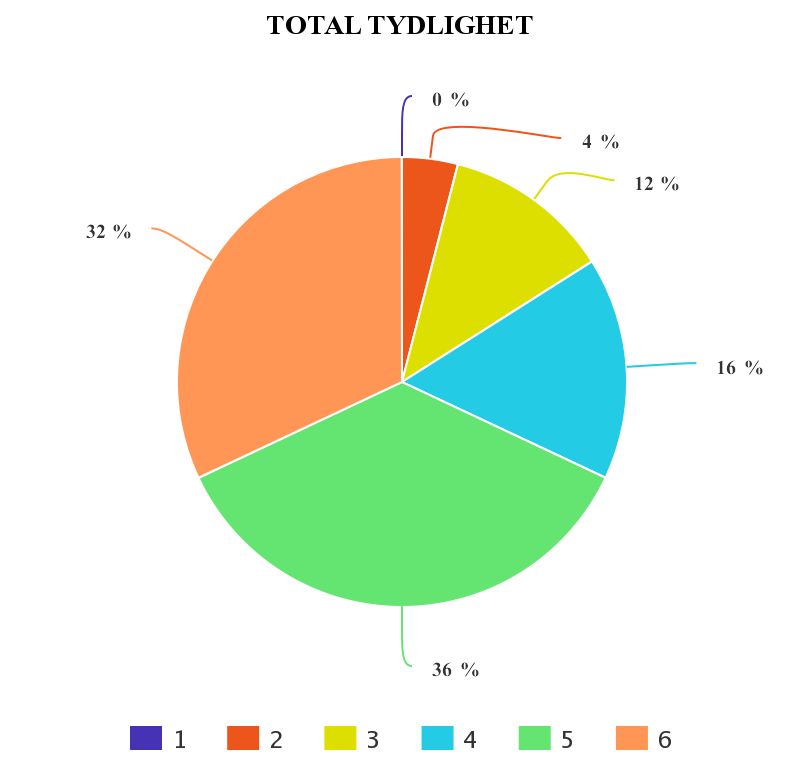
\includegraphics[scale=0.4]{meta-chart-2.png}
 \captionsetup{justification=centering,margin=2cm}
 \caption{Resultat av total tydlighet}
\end{figure} 



\begin{figure} [H]
  \centering
  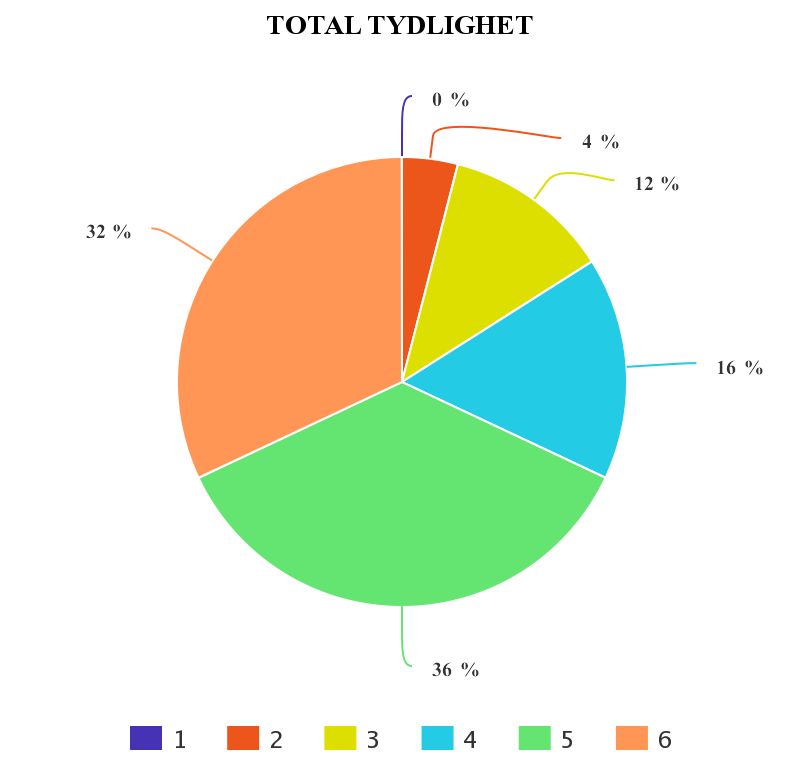
\includegraphics[scale=0.4]{meta-chart-2.png}
 \captionsetup{justification=centering,margin=2cm}
 \caption{Resultat av total tydlighet}
\end{figure} 

Figuren visar det slutgiltiga resultatet från både enkätundersökningen samt fokusgrupperna. Figuren visar sambandet mellan hur viktigt tydlighet är för användarupplevelsen i en applikation kontra hur tydlig prototypen känts. Den första rutan visar på hur viktigt det är för användaren att en applikation är tydlig, enligt personerna som medverkade i fokusgrupperna. Denna siffran beräknades med hjälp av snitt och varians och presenteras nedan. Diagrammen visar på hur tydlig prototypen kändes, enligt användarna som svarade på enkätundersökningen. 
\newline

\textbf{Citat från fokusgrupperna}
\begin{quotation}
\em Det var inte glasklart vart man ska markera, för det fanns ingen punkt eller checkbox
\end{quotation}

\begin{quotation}
\em Sen kan man ju tänka sig att ser man dåligt så är det lite för grått, texten är för grå.
\end{quotation}

\begin{quotation}
\em Man förstod att det var en film man skulle kolla på i och med att det var en playknapp. Inte svårt att förstå men jag fick inte sammanhanget. The why, varför gör jag detta, om jag får reda på det så kör jag vidare sedan utan att tänka.
\end{quotation}


%\begin{quotation}
%\em % hur många gånger ska jag göra de här övningarna? 
%\end{quotation}

%\begin{quotation}
%\em %Jag vill alltid tänka att ”vad är minimal effort för att gå vidare från detta”? 
%\end{quotation}

%\begin{quotation}
%\em %ja det är bra att se hur lång resan är. 
%\end{quotation}

%\begin{quotation}
%\em %Men det fanns ingen övergripande på dessa tre minuterna, det saknades ju helt. Det var på enskilda moment fanns det ju så att man kunde gissa sig fram på hur lång det var men inte helheten. 
%\end{quotation}

%\begin{quotation}
%\em %I think that it was not that clear, you have to be more clear in the beginning of what the goals for this exercise is. What is the goal and mission.  Why are you starting here? What is the steps? And I think it’s important to visualize it. 
%\end{quotation}


\newpage
\subsection{Effektivitet}

\centerline{\textbf{Hur viktigt är effektivitet för 
din användarupplevelse}}
\begin{figure}[H]
  \centering
  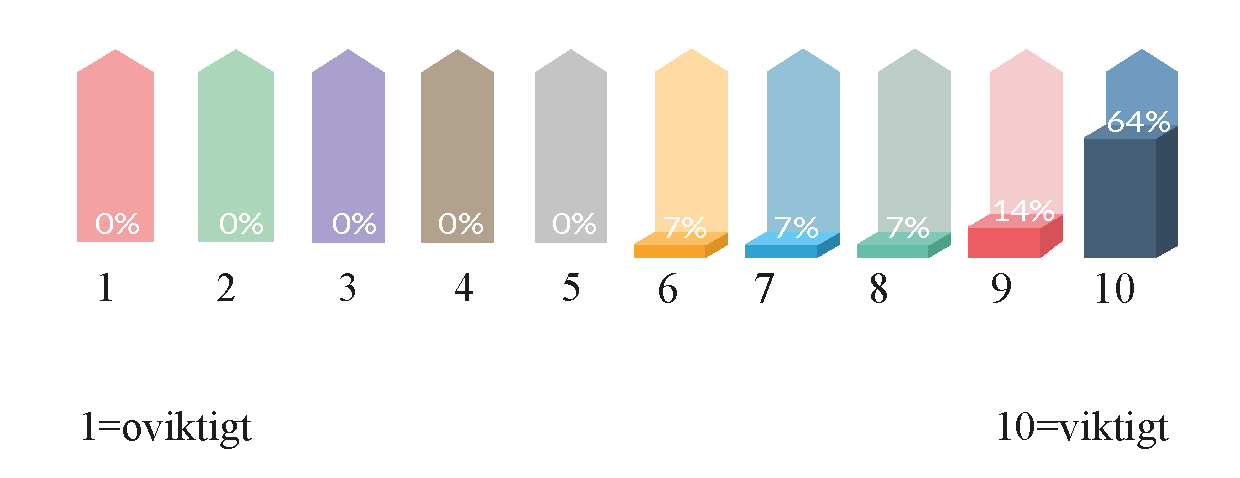
\includegraphics[scale=0.7]{Rityta_9.pdf}
\centering
\captionsetup{justification=centering,margin=2cm}
\caption{Resultat i procentuell skala på respondenternas svar}
\end{figure} 

Medelvärdet av ovan figur är 9.2. Siffran representerar ett medelvärde av stapeldiagrammet som visar hur viktigt det var för användarupplevelsen enligt kategoriseringen framtagen av Laugwitz et al. \cite{Laugwitz2008ConstructionQuestionnaire}.

%\[
 % m= 9.2
  %m = \frac{6+ 7+ 8 + 18 + 90}{14} = 9.2
  %\]

%Med en standardavvikelse på
%\[
 % \sigma = \sqrt{V} = \sqrt{ \frac{(6-1)^{2} + (7-1)^{2} + (8-1)^{2} + (9-2)^{2} + (10-9)^{2}} {5} } =  \sqrt{32} = 5.7
  %  \]

\begin{figure}[H]
  \centering
  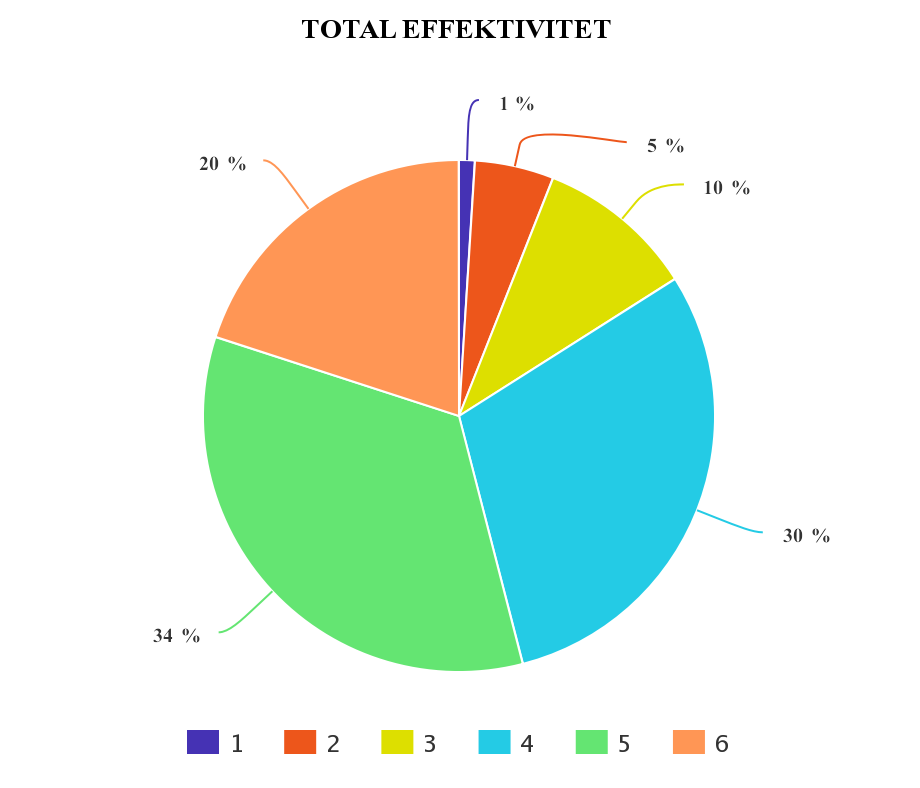
\includegraphics[scale=0.4]{meta-chart-3.png}
  \captionsetup{justification=centering,margin=2cm}
 \caption{Resultat av total effektivitet}
\end{figure} 
Figuren visar det slutgiltiga resultatet från både enkätundersökningen samt fokusgrupperna. Figuren visar sambandet mellan hur viktigt effektivitet är för användarupplevelsen i en applikation kontra hur effektiv prototypen känts. Den första rutan visar på hur viktigt det är för användaren att en applikation är effektiv, enligt personerna som medverkade i fokusgrupperna. Denna siffran beräknades med hjälp av snitt och varians och presenteras nedan. Diagrammen visar på hur effektiv prototypen kändes, enligt användarna som svarade på enkätundersökningen. 

\textbf{Citat från fokusgrupperna}
\begin{quotation}
\em Absolut är det viktigt att allting fungerar smidigt och att man kommer till nästa steg snabbt.
\end{quotation}

\begin{quotation}
\em  Effektivitet i alla former av digitala produkter är en självklarhet för mig. Ifall det buggar massvis hade jag inte orkat vara inne på applikationen och tagit det som att den inte är välgjort.
\end{quotation}

\begin{quotation}
\em Den tekniska delen är något man inte tänker på så mycket, man tar för givet att det ska fungera.
\end{quotation}


\newpage
\subsection{Pålitlighet}

\centerline{\textbf{Hur viktigt är pålitlighet för 
din användarupplevelse}}
\begin{figure}[H]
  \centering
  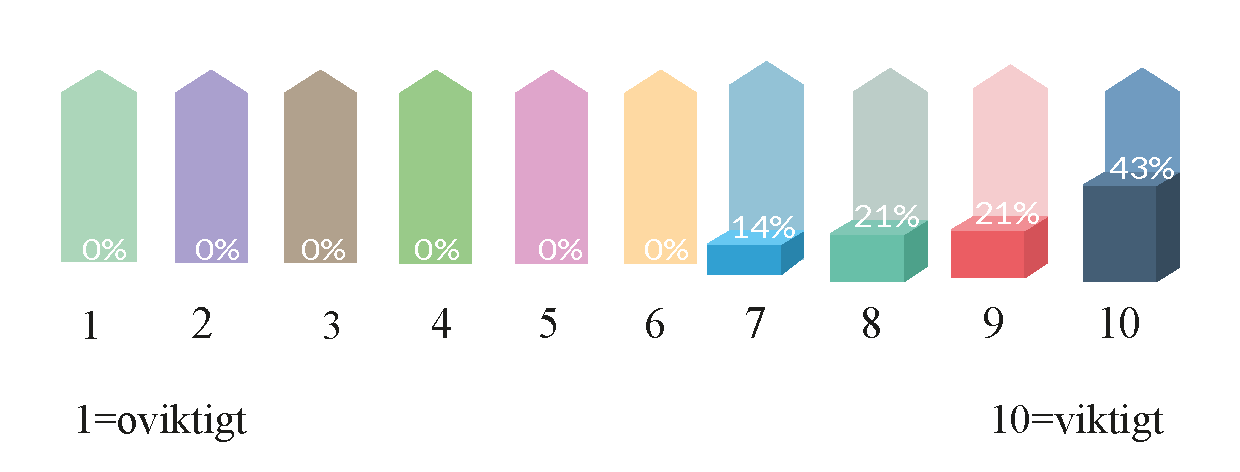
\includegraphics[scale=0.7]{Rityta_13.pdf}
  \centering
  \captionsetup{justification=centering,margin=2cm}
  \caption{Resultat i procentuell skala på respondenternas svar}
\end{figure} 

Medelvärdet av ovan figur är 8.93. Siffran representerar ett medelsnitt av stapeldiagrammet som visar hur viktigt det var för användarupplevelsen enligt kategoriseringen framtagen av  Laugwitz et al. \cite{Laugwitz2008ConstructionQuestionnaire}. 

%\[
%  m = \frac{14+ 24 + 27 + 60}{14} = 8.93
 % \]
  
%Med en standardavvikelse på

%\[
 %  \sigma = \sqrt{V} = \sqrt{  \frac{(7-2)^{2} + (8-3)^{2} + (9-3)^{2} + (10-6)^{2}} {4}} = \sqrt{25.5} = 5.1
  %  \]
\newpage   
\begin{figure}[H]
  \centering
  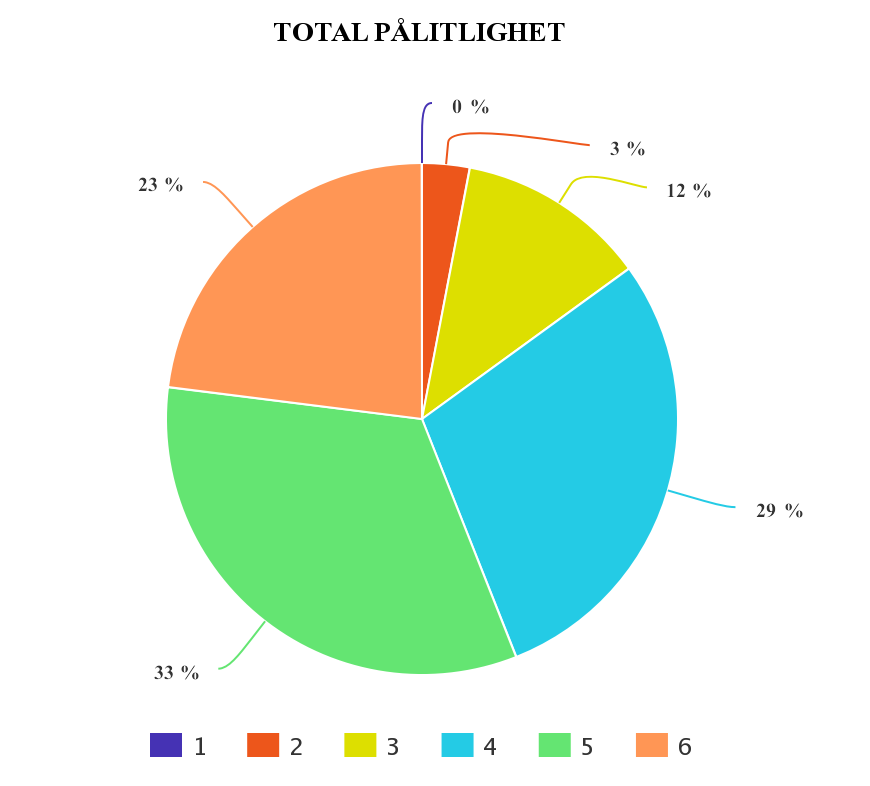
\includegraphics[scale=0.4]{meta-chart-4.png}
  \captionsetup{justification=centering,margin=2cm} 
  \caption{Resultat av total pålitlighet}
\end{figure} 

Figuren visar det slutgiltiga resultatet från både enkätundersökningen samt fokusgrupperna. Figuren visar sambandet mellan hur viktigt pålitlighet är för användarupplevelsen i en applikation kontra hur pålitlig prototypen känts. Den första rutan visar på hur viktigt det är för användaren att en applikation är pålitlig, enligt personerna som medverkade i fokusgrupperna. Denna siffran beräknades med hjälp av snitt och varians och presenteras nedan. Diagrammen visar på hur pålitlig prototypen kändes, enligt användarna som svarade på enkätundersökningen. 
    
\textbf{Citat från fokusgrupperna}
\begin{quotation}
\em Tex videon, den skulle behöva vara studioproducerad, känns lite ihopkok med telefonfilmen, det tappar trovärdighet. Alla detaljer behöver ha vass kvalité för att kännas trovärdig 
\end{quotation}

\begin{quotation}
\em I think that Ursulas tone is quite serious and she framför a serious message, but the prototype itself is not that serious, it’s a bit playful.  Because of the colors, it feels like a quiz which may not seem the most serious. 
\end{quotation}

\begin{quotation}
\em  You can mix playfulness and seriousness but if you have a lot of colors it don’t appear so serious.  But if you have one color and have that color along the journey it changes the user experience in a positive way and appear more serious. 
\end{quotation}

%\begin{quotation}
%\em %om jag får gå tillbaka till detta med attraktivitet så tycker jag att attraktivitet inte viktig för seriositeten, om detta hade varit min första interaktion med appen så ser den inte seriös ut, utifrån vad man är van vid och hur saker och ting ser ut designmässigt.
%\end{quotation}

%\begin{quotation}
%\em %Hjärnan fungerar som sådan att 40\% när vi gör saker går på autopilot, det betyder att vi använder oss av gamla vanor, dessa vanor skyddar oss från att testa nya saker. När något är för enkelt är det lättare att gå in i autopilot, gå in i en gamification snarare än att jag faktiskt reflekterar på riktigt. Och det är det svåra med sådana här typer av trainable app. 
%\end{quotation}

%\begin{quotation}
%\em %Det blir nog en utmaning att få till det i en kort video. Annars kommer man ju inte orka med att kolla. Hitta så att det blir seriös med inte för lång 
%\end{quotation}

%\begin{quotation}
%\em %Det var inte som ett spel för mig.  Jag saknade någon slags tydlig ram,  färgmässigt, lite stringent. Den känns lite ”fladdrig”. Det är viktigt att färgtemat följer en röd tråd och är sammanhängande.
%\end{quotation}

\newpage
\subsection{Stimuli}

\centerline{\textbf{Hur viktigt är stimuli för 
din användarupplevelse}}

\begin{figure}[H]
  \centering
  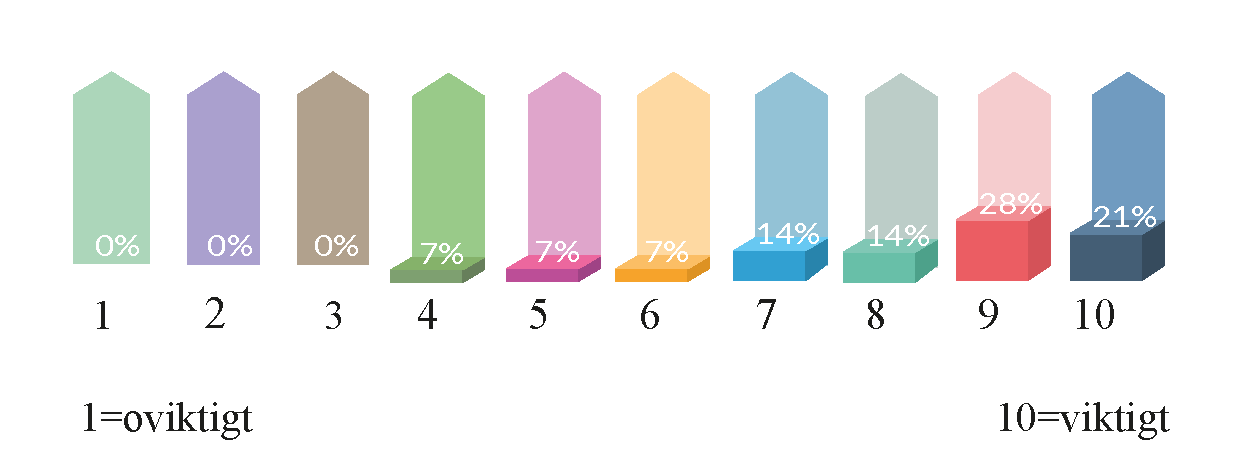
\includegraphics[scale=0.7]{Rityta_12.pdf}
  \centering
  \captionsetup{justification=centering,margin=2cm}
  \caption{Resultat i procentuell skala på respondenternas svar}
\end{figure} 

Medelvärdet av ovan figur är 7.93. Siffran representerar ett medelsnitt av stapeldiagrammet som visar hur viktigt det var för användarupplevelsen enligt kategoriseringen framtagen av Laugwitz et al \cite{Laugwitz2008ConstructionQuestionnaire}. 

%\[
 % m = \frac{4 +5 + 6 + 14 + 16 + 36 + 30}{14} = 7.93
 % \]
  
%Med en standardavvikelse på

%\[
 %\sigma = \sqrt{V} = \sqrt{ \frac{(4-1)^{2} + (5-1)^{2} + (6-1)^{2} + (7-2)^{2} + (8-2)^{2}+ (9-4)^{2} + (10-3)^{2} } {7}} \] 
 %\[
 %= \sqrt{26.43} = 5.14 \]

\newpage
\begin{figure}[H]
  \centering
  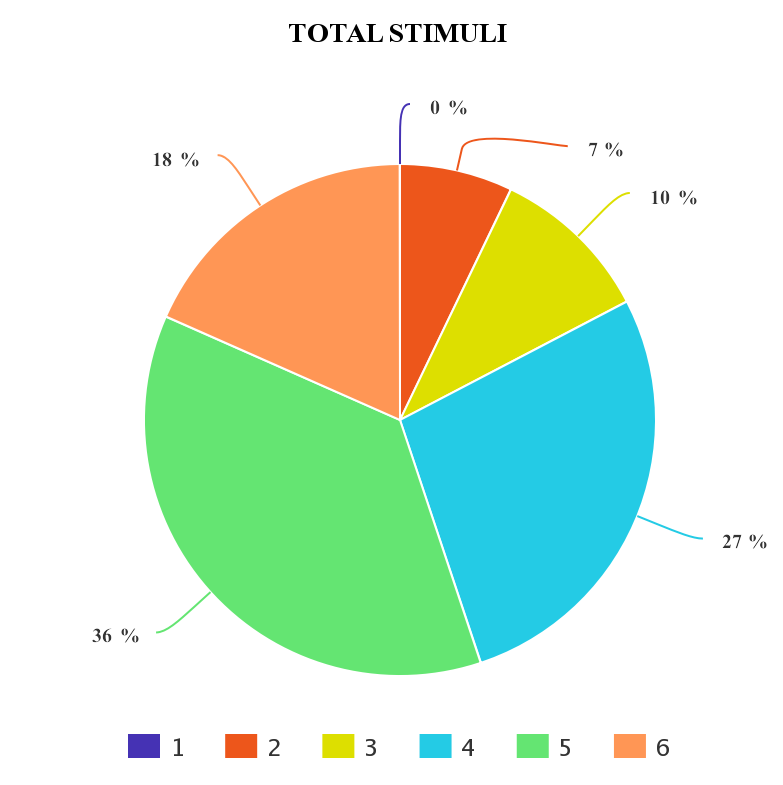
\includegraphics[scale=0.4]{meta-chart-5.png}
  \captionsetup{justification=centering,margin=2cm}
  \caption{Resultat av total stimuli}
\end{figure} 
Figuren visar det slutgiltiga resultatet från både enkätundersökningen samt fokusgrupperna. Figuren visar sambandet mellan hur viktigt stimuli är för användarupplevelsen i en applikation kontra hur stimulerande prototypen känts. Den första rutan visar på hur viktigt det är för användaren att en applikation är stimulerande, enligt personerna som medverkade i fokusgrupperna. Denna siffran beräknades med hjälp av snitt och varians och presenteras nedan. Diagrammen visar på hur stimulerande prototypen kändes, enligt användarna som svarade på enkätundersökningen. 

\textbf{Citat från fokusgrupperna}
%\begin{quotation}
%\em %vad har hänt innan appen? Vi säger om allt annat har fungerat så är appen inte viktig, jag skulle lägga mer krut på vad som är utanför appen snarare än vad som är inuti. 
%\end{quotation}

\begin{quotation}
\em  Utifrån hur Amazing Leaders jobbar här och nu så tror jag att det kan vara ett bra stöd, som en brygga in och för att få kontinuitet
\end{quotation}

\begin{quotation}
\em  Jag gillade interaktivitet i den, och att det var interaktivitet som var personlig för mig. Det tror jag är nyckeln, att det inte är generellt för alla, göra något och reflektera är viktigt. 
\end{quotation}

\begin{quotation}
\em Skulle nog vilja att det fanns en fördjupningsknapp om man ex skulle vilja läsa mer om vad EQ var, vad menas med vad som var mina actions. Då får man ännu en nivå på det 
\end{quotation}

%\begin{quotation}
%\em %Om vi har haft ett möte med, säg Ursula nu då, så har vi dessa tre aktiviteter och övningar som vi har på papper och som vi kan följa upp.
%\end{quotation}

%\begin{quotation}
%\em  %Den andra biten som jag tror kan va intressant också är den här resultat effekten, nån action därefter. vi säger det här kontraktet du har gjort i nån form utav fysiks dialog, dokumentationen och exekveringen utav det långsiktiga är något man kan bocka av.
%\end{quotation}


%\begin{quotation}
%\em %The app should support growth so it does not have to be fun, maybe it should not be fun, then it won’t be serious. It should tot boring but not like a game either. 
%\end{quotation}


\newpage
\subsection{Attraktivitet}


\centerline{\textbf{Hur viktigt är attraktivitet för 
din användarupplevelse}}

\begin{figure}[H]
  \centering
  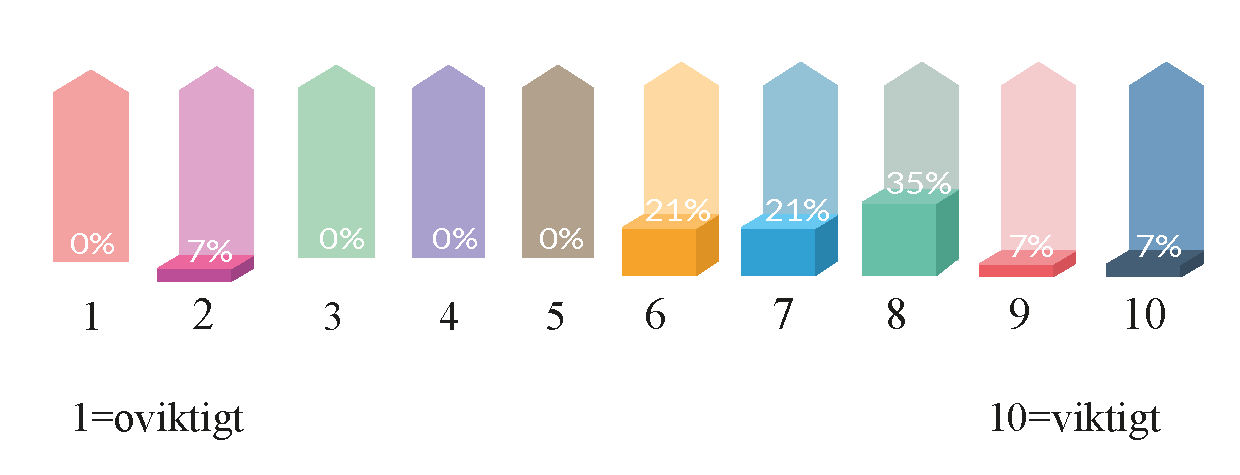
\includegraphics[scale=0.7]{Rityta_11.pdf}
 \captionsetup{justification=centering,margin=2cm}
\caption{Resultat i procentuell skala på respondenternas svar}
\end{figure} 

Medelvärdet av ovan figur är 7.14. Siffran representerar ett medelsnitt av stapeldiagrammet som visar hur viktigt det var för användarupplevelsen enligt kategoriseringen framtagen av Laugwitz et al. \cite{Laugwitz2008ConstructionQuestionnaire}. 

%\[
 % m = \frac{2 + 18 + 21 + 40 + 9 + 10}{14} = 7.14
%  \]
  
%Med en standardavvikelse på

%\[
%\sigma = \sqrt{V}= \sqrt{\frac{(2-1)^{2} + (6-3)^{2} + (7-3)^{2} + (8-5)^{2} + (9-1)^{2} + (10-1)^{2}} {6}} = \sqrt{30} = 5.5
 %   \]

\newpage
\begin{figure}[H]
  \centering
  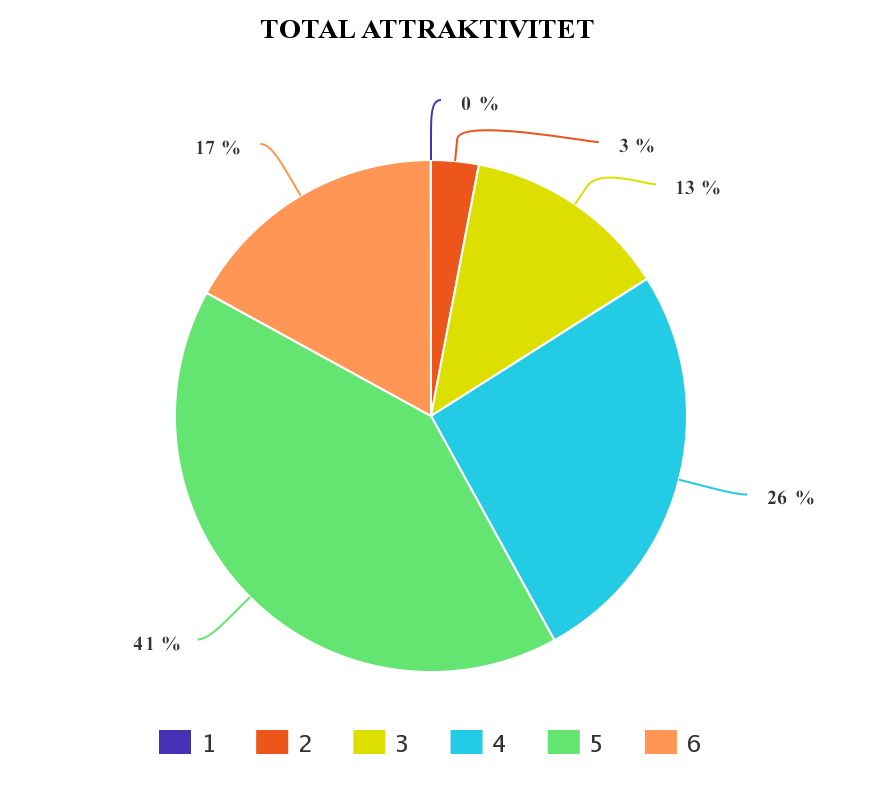
\includegraphics[scale=0.4]{meta-chart-6.png}
 \captionsetup{justification=centering,margin=2cm}
  \caption{Resultat av total attraktivitet}
\end{figure}

Figuren visar det slutgiltiga resultatet från både enkätundersökningen samt fokusgrupperna. Figuren visar sambandet mellan hur viktigt attraktivitet är för användarupplevelsen i en applikation kontra hur pålitlig prototypen känts. Den första rutan visar på hur viktigt det är för användaren att en applikation är attraktiv, enligt personerna som medverkade i fokusgrupperna. Denna siffran beräknades med hjälp av snitt och varians och presenteras nedan. Diagrammen visar på hur attraktiv prototypen kändes, enligt användarna som svarade på enkätundersökningen. 
\newline

\textbf{Citat från fokusgrupperna}
\begin{quotation}
\em  Det var tydligt och rent, det var lätt att komma igång med det. Lättillgängligt. 
\end{quotation}

\begin{quotation}
\em  Jag tycker att den är inbjudande för att den är enkel och det är inte jättemycket textmassor utan det är ganska instinktivt hur jag ska börja klicka
\end{quotation}

\begin{quotation}
\em  I think it looked really nice, but I think its a bit hard to understand whats the mission is. And I think that if you could show it in a graphical way before she start to tak, other wise its hard to get the point.  But I think it’s nice to have someone talking for once, because usually it’s a lot of text and so.
\end{quotation}

%\begin{quotation}
%\em %Vill alltid ha kontroll på hur långt jag kommit, så det är bra. Vill veta vart är jag, hur mycket har jag kvar, är det lönt att börja på en ny osv.
%\end{quotation}

%\begin{quotation}
%\em  %Det var lagom långa filmer, så fort dom blir för långa så tappar jag uppmärksamheten.
%\end{quotation}

%\begin{quotation}
%\em  %Ja nu vet jag ungefär vad jag har att förvänta mig och därför har jag hög acceptansnivån för utseendet 
%\end{quotation}

%\begin{quotation}
%\em   %Man kanske kan paketera det lite grann så att det inte blir så internt coach perspektiv.
%\end{quotation}

%\begin{quotation}
%\em %Kanske att man distribuerar det eller att du får möteskallelser automatiskt in i telefonen för att faktiskt göra dessa actions som du kommit överens
%\end{quotation}

%\begin{quotation}
%\em  %Ja det var verkligen lagom långt klipp
%\end{quotation}

%\begin{quotation}
%\em %Då är det bra att det finns en tidslinje, så man ser hur långt den är
%\end{quotation}

%\begin{quotation}
%\em %För just videon signalerar ju någon form utav personlig dialog. Men om det bara är en allmän instruktion som är lika oavsett vad jag svara i olika steg så är den kanske lite besviken på den. 
%\end{quotation}

%\begin{quotation}
%\em  %Inte så mycket ”buzz”. Det är funktion snarare än att det är feeling. Det är inte så säljande, inte så wowigt, inte så mycket konfetti, utan det är funktion.
%\end{quotation}

%\begin{quotation}
%\em %I liked that it had clear intentions, very specific for the person who uses it. And a clear flow of the prototype. But I would like an option to skip the videos and have a text or something. 
%\end{quotation}


\newpage
\section{Generell rekommendation och sammanställning}

\subsection{Vad vi kan rekommendera som nästa riktning}
Från resultatet ser man att de olika kategorierna har relativt varierande svar. Det är överlag höga betyg för kategorierna. Rangordningen var
% Som!man!kan!se!i!diagrammen!får!de!olika!kategorierna!relativt!enhetliga!svar.!Det!är!
% överlag!höga!betyg!för!samtliga!kategorier!men!man!kan!också!se!skillnader!mellan!de!
% hedonistiska!–!och!användbarhetskategorierna.!För!de!hedonistiska!kategorierna!ligger!
% antal!svar!på!fem!(5)!och!sex!(6)!på!totalt!43%!respektive!53%,!medan!de!för!
% användbarhetskategorierna!ligger!på!70%,!61%!respektive!64%.!Detta!ser!vi!som!en!
% indikator!på!att!användbarheten!för!systemet!bedöms!som!bättre,!av!de!svarande,!än!de!
% hedonistiska!kategorierna!gör.!

\subsection{Resultat från utvärdering av prototyp}
Överlag hade användaren en positiv bild av AL1. Vad fokusgrupperna diskuterade
\\
% se: http://www.csc.kth.se/utbildning/kandidatexjobb/teknikmanagement/2010/rapport/jensen_anna_OCH_persson_johan_K10052.pdf

Datan visar på att tydlighet är viktigast. På prototypen ansåg de flesta att den var bra. Trots det var det 4 och 12 procent som tyckte den var svår att förstå och komplicerat. 
Från fokusgrupperna förstod man att medlemmarna inte tyckte det var \enquote{glasklart} vart man skulle markera. 
\\
Till en början rekommenderar vi att man 

När man då tittar på vad fokusgrupperna sa var

\newpage
\section{Diskussion}
\label{sec:discussion}
I det här avsnittet diskuteras resultatet av studien. Först presenteras avgränsningarna av studien och dess inverkan på studien. Efter det diskuteras kvaliteten av resultaten följt av vad man kunde ha gjort bättre. 

\subsection{Avgränsningar av studien}
En stor begränsning av studien har varit målgruppen till utvärderingen. Då Amazing Leaders inte fastställt hur deras framtida applikation skulle vara så var det svårt att kunna definiera vilka slutanvändaren skulle vara. För att få en så bra uppfattning som möjligt var målet med studien att få en stor bredd av deltagare till utvärderingarna. Det gjordes en avgränsning där enkätundersökningen målgrupp begränsades till personer inom befintliga organisationer och företag som vill lära sig mer om EQ. Urvalet för fokusgrupperna blev istället baserat på vissa kriterier (se mer om detta i avsnitt Målgrupp \ref{malgrupp}). Den här avgränsning hade en effekt på resultatet då de som var intresserade att göra enkätundersökningens inte var så många. Det har förstått att de som är intresserade för att bli \enquote{EQ-smart} var bara en begränsad grupp där även andra kunde vara möjliga slutanvändare som kunde genomföra enkätundersökningen.
\\

En annan avgränsning var att inte utvärdera användbarhet utan endast user experience. Det gjorde att vi i den mån vi hann försökte förbättra prototypens funktionalitet men att det inte var i studiens omfång. Denna begränsning gjorde att vissa funktionaliteter inte var möjliga att evaluera och det var problematiskt att försöka förklara vad skillnaden mellan användbarhet och user experience var. Trots att detta förklarades i syftet och inbjudan till utvärderingarna är det möjligt att respondenterna inte förstod skillnad vilket skulle minska reliabiliteten av resultatet.
\\

En annan parameter som var en avgränsning för studien var valet av ramverk. Vid början av litteraturstudien förstods det snabbt att det fanns många definitioner av UX och nästan lika många ramverk. Vid val av ramverk gjordes en grundlig litteraturstudie som bestämde vilket ramverk som lämpade sig bäst för studiens mål. En aspekt som kan ha förändrat hela studiens omfattning och resultat är valet av ramverk.

\subsection{Kvalitet}
För att öka kvaliteten av den insamlade datan användes ljudinspelning för fokusgrupper, som sedan transkiberades på detaljnivå. Detta reducerar möjligheten för missförstånd vid analys av data, och gör att en kvalitet kan bli försäkrad.
\\

Utöver detta reviderades frågorna till enkätundersökningen och fokusgrupperna ett flertal gånger för att försäkra sig om att deltagarna och respondenten tolkade frågan på exakt samma sätt. Det eliminerade möjliga frågetecken och tolkningsfel vid svar av enkätundersökningen. 
\\

En aspekt som påverkat studien är antalet respondenter under både enkätundersökningar och fokusgrupper. Under arbetets korta tidslinje har respondenterna över lag varit väldigt bra, då de har valt på ett sätt så att de är i rätt målgrupp. Någon som däremot skulle kunna förbättra den totala kvaliteten på både befintligt och framtida arbete är om antalet enkät- och fokusgrupps- deltagare kunde ökas. Detta då man skulle kunna introducera nya analysområden, så som statistiskt underlag samt att kunna validera resultaten på ett mer gediget sätt. 
\\

För att kunna göra detta skulle man även behöva omformulera enkäten på ett sätt så att det skulle vara mer lämpad för djupare analys. 
\\

\subsection{Förbättringsområde}
En del av arbetet tillsammans med uppdragsgivaren var att etablera målgrupp och avgränsa arbetet. Om denna tid kunde allokeras till annat hade det varit fördelaktigt för studien i sin helhet då det skulle öppna upp tidsplaneringen. \\

Det hade varit bra om man ser igenom enkäten för att se hur man kan förändra och förbättra den för att extrahera mer information. Det är svårt att göra en bra analys då den data man får in är en skala från 1-6. Man skulle till exempel kunna be respondenterna rangordna kategorierna. Då skulle man kombinatoriskt kunna se vad folk tycker är viktigast.\\

Studien använde fokusgrupper för att få kompletterande och komplett data. Ett förbättringsområde även där hade varit att se över genomförandet av fokusgrupper för att få ut mer ur den timmen som var avsatt för diskussion i fokusgruppen. 

\newpage
\section{Slutsats och framtida forskning}



\section{Framtida Forskning}

\newpage
\printbibliography
\newpage
\onecolumn
\newpage

\appendices
\section{Fokusgrupper}
\subsection{Fokusgrupp 1} 

\textbf{Transkriberad ljudinspelning från Fokusgrupp 1} \\

Anna: Vad tycker ni om det allmänna utseendet av prototypen? \\

Person 5: Jag måste bara säga en sak innan vi kastar oss in i den frågan. Det beror mycket på hur mycket vetskap man har innan man använder den här sidan, det är avgörande tror jag. Jag tycker själv såhär .. Ja nu vet jag ungefär vad jag har att förvänta mig och därför har jag hög acceptansnivån för utseendet. Om det ska vara en catchy-säljigt sida då tror jag att det finns jobb att göra, det är mitt inspel på det. Vem är jag, vart kommer jag ifrån, är det någon sökning på nätet som jag har hittat hit eller svenska spel som har gjort en stor upphandling av kurser? Sånt behöver man veta innan man sätter sig in i denna rollen. För mig har det bäring på det med utseendet och sådär. Ska det vara säljigt eller bara funktionellt? Så säligt är det inte tycker jag, mer funktionellt. 

Person 2: Jag tycker att den är inbjudande för att den är enkel och det är inte jättemycket textmassor utan det är ganska instinktivt hur jag ska börja klicka. Det finns en pil där jag ska trycka, och det är ganska  intuitivt att veta när jag ska komma igång. Inte jättemycket text vilket jag tycker är bra, bilder färger. Inte så att jag blir förvirrad över var jag ska börja. Sen vet jag inte om den är speciellt inbjudande.\\

Person 1: Jag blir lite fundersam när man tittar på första sida, \enquote{learning EQ och self leadership}, det är ju lite gran den lingon som är inom ledarskaps utveckling. Man kanske kan paketera det lite grann så att det inte blir så internt coach perspektiv. För jag gillar att ha slutprodukten synlig, som något slags kontrakt. Sen kan man fundera på vad man kan göra med den för att befästa den. Oavsett om du har kommit in i den här processen inom att vara i en mobil värld eller i en fysisk dialog så har man ungefär skapat samma kontrakt. Den som är tricket här är att få det levande över en tid och då måste du kanske befästa detta kontraktet på något sätt, kanske att man distribuerar det eller att du får möteskallelser automatiskt in i telefonen för att faktiskt göra dessa aktions som du kommit överens. \\

Person 5: Det är bra  med kort information, instruktion, inga sådana här tio minuters lyssningar. \\

Person 2: Ja det var verkligen lagom långt klipp. Jag tänkte på när man klickar in där så hamnar man mitt inne i två av tio lektioner. Då är det bra att det finns en tidslinje, så man ser hur långt den är. Jag skulle nog ha en annan förstasida oavsett vart den landar.\\

Person 1: Jag gillade det personliga tilltalet i videon. Sen kan man fundera på om man i processen kan få ännu mer personligare. I början är det okej att det är generellt, utan någon personlig information. För just videon signalerar ju någon form utav personlig dialog. Men om det bara är en allmän instruktion som är lika oavsett vad jag svara i olika steg så är den kanske lite besviken på den. \\

Person 5: Jag gillar att det var funktionellt, här ska man trycka, man har inte så mycket andra initiativ eller möjligheter. Inte så mycket ”buzz”. Det är funktion snarare än att det är feeling. Det är inte så säljande, inte så wowigt, inte så mycket konfetti, utan det är funktion.. tryck här och sedan gå vidare. Det behöver inte vara fel men det är min känsla. \\ 

Anna: Är det lätt att förstå vad du ska göra som användare? hur många gånger ska jag göra de här övningarna? \\

Hela gruppen: Ja\\

Person 2: Se så ser man inte pilen förrän man trycker på skärmen, utan man ser bara en bild, då tycker man -har man fastnat nu eller. \\

Person 5: Jag tycker det är självklart när man markerar, här på MAC datorn, det man vill klicka på så blir det ett förstoringsglas. Det var inte glasklart vart man ska markera, för det fanns ingen punkt eller checkbox, ska jag klicka på texten här eller.. Det var inte super tydligt. \\

Person 2: Sen kan man ju tänka sig att ser man dåligt så är det lite för grått, texten är för grå. Så jag får ju då använda förstoringsglas \\

Person 5: Kan man göra en sådan här grej att vid markeringen där när man hovrar över texten så går fonten upp. Bara så att man ser \\

Person 4: Är inte det super irriterande? \\

Person 5: Bara för att markera, \enquote{här är du} liksom. \\

Person 4: MAC:en har ju en docka här nere med applikationer och sedan så ett förstoringsglas, det är det första man stänger av så den inte håller på att förstora och förminska. Men det är ju en annan liknelse. \\

Anna: Men var det lätt för dig att förstå vad som var nästkommande steg?\\

Person 4: Nej jag tycker inte det, det var oklart. Det första jag funderar över som förmodligen förklaras någonstans, är varför lifeintentions är viktigt. Det förklarades inte tyckte jag. Sen så är det då när man svarar och gå vidare,Men det var ju enkelt i form av att jag inte kunde gör något annat mer än att gå vidare. Inte min effort i form av okej nu har jag gjort detta, vad kommer sendan? \\

Anna: Skulle du känna att du skulle vilja se det, hur många steg du vill göra i övningen? \\

Person 4: Nu är det väldigt påverkad av hur vi tänker kring UX design på klarna, och det är solklart att det alltid ska vara så. Jag vill alltid tänka att \enquote{vad är minimal effort för att gå vidare från detta}? \\

Person 5: ja det är bra att se hur lång resan är. \\

Person 1: det var ju någon form utav en progressiv indikator, när man svarade på dessa flervalsfrågorna, det var ju bra! Men det fanns ingen övergripande på dessa tre minuterna, det saknades ju helt. Det var på enskilda moment fanns det ju så att man kunde gissa sig fram på hur lång det var men inte helheten. \\

Person 3: men ja tkr också total sammanställningen är viktig. \\

Anna: Känns appen trovärdig?\\

Person 4: om jag får gå tillbaka till detta med attraktivitet så tycker jag att attraktivitet inte viktig för seriositeten, om detta hade varit min första interaktion med appen så ser den inte seriös ut, utifrån vad man är van vid och hur saker och ting ser ut designmässigt. 
Det finns en app, som man kan klassa som en konkurrent, där man går igenom appen och går igenom sina grundvärderingar utifrån forskning så är det ett väldigt stort antal värderingar. Det tar mer effort, så jag värderar att resultatet mer i och med att det tar mer effort, så ju snabbare det går, desto mindre seriös och med som pop-quiz på Facebook. Appen ser extremt proffsig ut i jämförelse med prototypen. Men också sättet man sortera ut känns mer seriöst när det finns mer val, och jobbigare. Och problemet, när vi har testat ai-coachning, är hur människor fungerar. Hjärnan fungerar som sådan att 40 procent när vi gör saker går på autopilot, det betyder att vi använder oss av gamla vanor, dessa vanor skyddar oss från att testa nya saker. När något är för enkelt är det lättare att gå in i autopilot, gå in i en gamification snarare än att jag faktiskt reflekterar på riktigt. Och det är det svåra med sådana här typer av trainable app. \\

Anna: Hur modern kändes denna prototypen?\\

Person 4: inte alls, för att finns ingenting nytt i den, sättet att lära ut på , nä de är jättemånga som gör det, samma sak med video. Jag vet inte vad som skulle vara nytt över huvud taget.\\

Anna: Men kändes den stimulerande att använda?\\

Person 4: Jag tror att för mig, som har testat jättemånga sådana appar och försökt implementera det, det börjar inte med appen, det börjar i en annan ända, vad har hänt innan appen? Vi säger om allt annat har fungerat så är appen inte viktig, jag skulle lägga mer krut på vad som är utanför appen snarare än vad som är inuti.\\ 

Person 3: Jag tänker att det är en bra förlängning då, att man har detta som ett komplement till nästa steg. Utifrån hur Amazing Leaders jobbar här och nu så tror jag att det kan vara ett bra stöd, som en brygga in och för att få kontinuitet. \\

Person 5: Ja, för att föra folk framåt, utan att varje gång behöva träffas. Mekanism för att driva utvecklingen för individerna framåt. Om vi har haft ett möte med, säg Ursula nu då, så har vi dessa tre aktiviteter och övningar som vi har på papper och som vi kan följa upp.\\ 

Person 1: Jag är inne på samma sak, man behöver nästan bestämma sig, antingen så är det förberedande och då är det inte seriositet så viktigt, då är det mer ett insamlingsmoment. Skriv ned dessa 10 saker i din bok, de där har man ju väldigt svårt att ta sig för. Detta skulle kunna vara ett enkelt sätt för att jag inte ska behöva gå tillbaka till mina anteckningar. Den andra biten som jag tror kan va intressant också är den här resultat effekten, nån action därefter. vi säger det här kontraktet du har gjort i nån form utav fysiks dialog, dokumentationen och exekveringen utav det långsiktiga är något man kan bocka av. Lite som gamificaition, jag har gjort detta, det som vi kom överens om. \\

\subsection{Fokusgrupp 2}

\textbf{Transkriberad ljudinspelning från Fokusgrupp 1}
\\

Anna: Vad tycker ni om det allmänna utseendet av prototypen? \\

Person 1: Jag gillade det på första sidan, detta med att det ser ut som en scroll. Så att man kan se progressen. Vill alltid ha kontroll på hur långt jag kommit, så det är bra. Vill veta vart är jag, hur mycket har jag kvar, är det lönt att börja på en ny osv. \\

Person 4: Det är nästan så man skulle vilja se vilket kapitel och hur lång övningen är, så man förstår vad man ger sig in på. \\

Person 1: Men bara som någon slags förstaupplevelse, vart är jag för någonstans? \\

Var prototypen inbjudande?\\

Person 3: ja det tycker jag. Det var tydligt och rent, det var lätt att komma igång med det. Lättillgängligt. \\

Person 2: Jag är oftast väldigt rastlös när man tittar i en telefon, vill se direkt vad det är, inte så mycket text utan det ska vara tydligt och enkelt. Förstår direkt vad det är man gör. \\

Person 1: Ja precis, lite det här med att less is more. Få grejer men man ska direkt förstå vad som ska göras. \\

Person 3: Det var lagom långa filmer, så fort dom blir för långa så tappar jag uppmärksamheten. \\

Person 3: Gå framåt och bakåt saknade jag \\

Person 1: Första sidan var bra, men att man får mer kontroll. Man såg att det var en film men det gick inte se hur lång den var, men jag vill veta hur lång den är. Om det är andra gången jag går in så vill jag dra fram 45 sekunder om jag redan har sett på det. \\

Hur tydlig var prototypen? \\

Person 3: Man kände att det var en prototyp, just för att dessa småsaker var inte mer. Blir mer nyfiken på hur nästa version kommer att vara \\

Person 1: Sådär, för att den känns lite buggig. \\

Person 4: det var inte riktigt tydligt hur man skulle klicka klart tycker jag. Lite mer intuitivt \\

Vad det lätt att förstå vad som förväntades? \\

Person 3: Man förstod att det var en film man skulle kolla på i och med att det var en playknapp. Inte svårt att förstå men jag fick inte sammanhanget. The why, varför göra detta, om jag får reda på det så kör jag vidare sedan utan att tänka.\\

Person 4: Inte riktigt tydlig kontext. \\

Förstod man vad som var nästkommande steg?\\

Person 1: ja men det tycker jag, man tog ju sig framåt för att det inte fanns så många andra alternativ. \\

Person 3: Jag gillade att det var lika dana blåa bars. Den blå knappformen hjälpte tydligheten. Man fattade att det var en form av action. \\ 

Hur pålitlig kändes prototypen?\\

Person 2: Det blir nog en utmaning att få till det i en kort video. Annars kommer man ju inte orka med att kolla. Hitta så att det blir seriös med inte för lång \\

Person 1: Tex videon, den skulle behöva vara studioproducerad, känns lite ihopkok med telefonfilmen, det tappar trovärdighet. Alla detaljer behöver ha vass kvalité för att kännas trovärdig \\

Hur modern kändes prototypen? \\

Person 3: Sådär, det finns ju mycket sånt men den kändes trevlig, mer trevlig än nytänkande typ. \\ 

Person 2: Ja precis, jag håller med.\\

Person 1: Gillar första sidan, den var fräsch. \\

Person 3: Den här blir mer personlig än om det bara skulle vara grafiskt. \\

Kändes den stimulerande? \\

Person 1:  Jag gillade att  interaktivitet i den, och att det var interaktivitet som var personlig för mig. Det tror jag är nyckeln, att det inte är generellt för alla, göra något och reflektera är viktigt. \\

Person 3: Skulle nog vilja att det fanns en fördjupningsknapp om man ex skulle vilja läsa mer om vad EQ var, vad menas med vad som var mina actions. Då får man ännu en nivå på det \\

\subsection{Fokusgrupp 3}

\textbf{Transkriberad ljudinspelning från Fokusgrupp 3} \\

Person 1: I liked that it had clear intentions, very specific for the person who uses it. And a clear flow of the prototype. But I would like an option to skip the videos and have a text or something. \\

Person 3: I think it looked really nice, but I think its a bit hard to understand whats the mission is. And I think that if you could show it in a graphical way before she start to tak, other wise its hard to get the point.  But I think it’s nice to have someone talking for once, because usually it’s a lot of text and so.\\

Person 4:  I agree with both of you,  and the interface Is okay.  In the whole scope it’s good. But I would like to have a functionality to go back and maybe repeat, if you come up with something more that you would write for your answer. \\

Person 5 : I really liked the person person who talked, she was calm.  The flow is structured well. \\

Person 3: Another thing; maybe it should visualize the total journey, like, I’m here right now, I started there and this is the end.  It’s very important to understand the mission, the goal and why, how , what and where I am right now. \\

Person 1: Yes, you want to se progress of what you are doing. But you don’t have to be forced to do it , if you want to see your progress you can do it. \\

Person 5: Maybe it can be a bar that you could hide if you don’t want to see the progress. \\ 

Person 2: I liked the design, I think that colors is nice, easy with the flow. I understand what to do. Then I agree on the alternative to the video, maybe show a text , if you don’t able to have sound. And a progress bar Is nice to see where you have started and were you going, so you could orient yourself a bit were you are. \\

Person 3: I think that it was not that clear, you have to be more clear in the beginning of what the goals for this exercise is. What is the goal and mission.  Why are you starting here? What is the steps? And I think it’s important to visualize it. \\ 

Person 1: The app is clear, but If I have a goal how would I know that the app is helping me reach that goal? When I’m in the app and chosen my intentions, that is clear my question is that, does it help me in any way? \\

Person 3: its not clear what the purpose is and if the app helps me. \\ 

Person 2: I think that Ursulas tone is quite serious and she framför a serious message, but the prototype itself is not that serious, it’s a bit playful.  Because of the colors, it feels like a quiz which may not seem the most serious. \\

Person 5: I think it was serious, because of the message she gave. It was reliable, didn’t think that I was playing. \\ 

Person 2: Det var inte som ett spel för mig.  Jag saknade någon slags tydlig ram,  färgmässigt, lite stringent. Den känns lite ”fladdrig”. Det är viktigt att färgtemat följer en röd tråd och är sammanhängande. Behövs lite mer tydligt att det finns en huvudmeny, om man vill backa eller om man vill pausa.  Det är svårt att svara på frågan om den är pålitlig då prototypen buggade, fick en känsla av att den lite var pålitlig då.  Fungerar inte tekniken så hoppar jag över det, det är jätteviktigt för mig. Det hade varit bra om man fick skriva noteringar eller frågor som jag har till min coach, antingen separat eller kopplat till mitt coachingpnogram. \\

Person 1: What she said about the color scheme, you can mix playfulness and seriousness but if you have a lot of colors it don’t appear so serious.  But if you have one color and have that color along the journey it changes the user experience in a positive way and upper more serious. \\

Person 3: I’ts not fun, but must it be fun? I’m not certain that it should be fun actually.  This is something for me and my journey, mor of an stimulation in that context. \\

Person 3: Stimulation for me is something that I can use in my daily life or at home. For me its a good thing if I can see that I have a benefit from it. \\

Person 3: The app should support growth so it does not have to be fun, maybe it should not be fun, then it won’t be serious. It should tot boring but not like a game either. \\

Person 4:  Personally I would only like to have that once, or else I just cancel the message or don’t read it. \\

Person 2: The fact that we know that she is an experienced coach it makes the app more reliable. But if you don’t know that she can say it in the beginning of the video. \\
\section{Enkätundersökning}

    
 \begin{figure} [H]
   \centering
   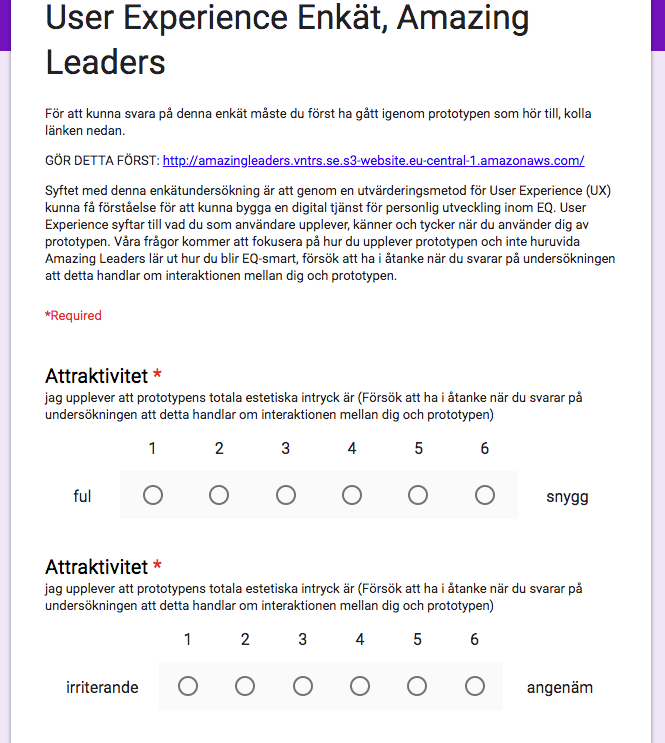
\includegraphics[scale=0.75]{form1.png}
  \captionsetup{justification=centering,margin=2cm}
  \caption{Enkätundersökning}
 \end{figure} 
 
  \begin{figure} [H]
   \centering
   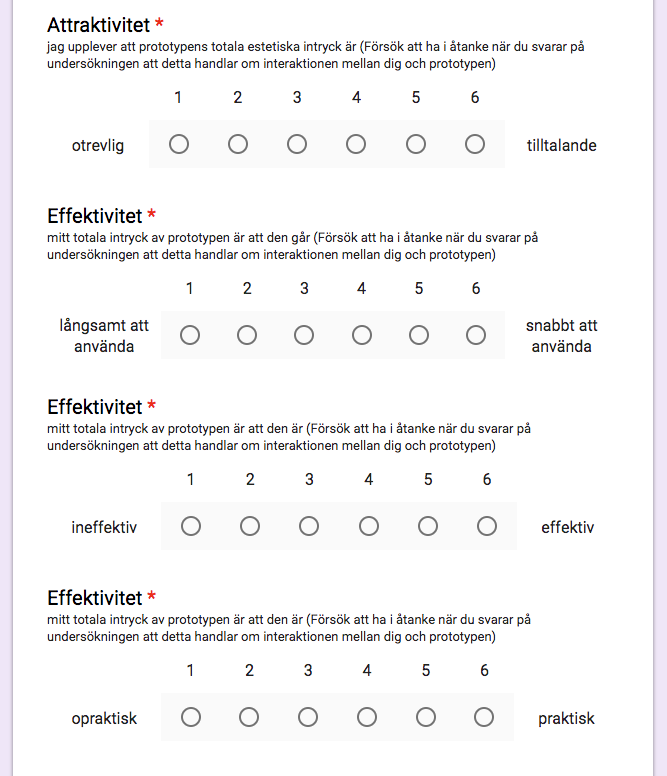
\includegraphics[scale=0.75]{form2.png}
  \captionsetup{justification=centering,margin=2cm}
  \caption{Enkätundersökning}
 \end{figure} 

 \begin{figure} [H]
   \centering
   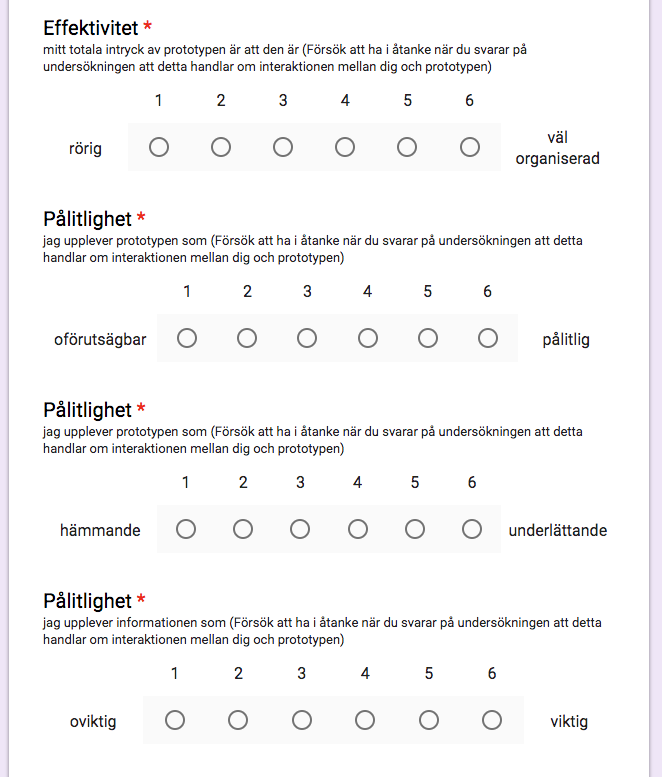
\includegraphics[scale=0.75]{form3.png}
  \captionsetup{justification=centering,margin=2cm}
  \caption{Enkätundersökning}
 \end{figure} 
 
  \begin{figure} [H]
   \centering
   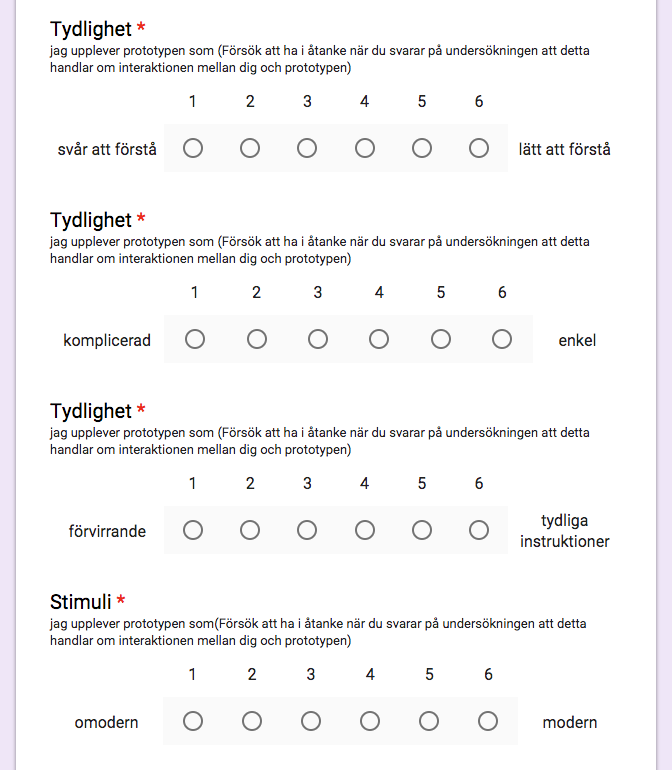
\includegraphics[scale=0.75]{form4.png}
  \captionsetup{justification=centering,margin=2cm}
  \caption{Enkätundersökning}
 \end{figure} 
 
  \begin{figure} [H]
   \centering
   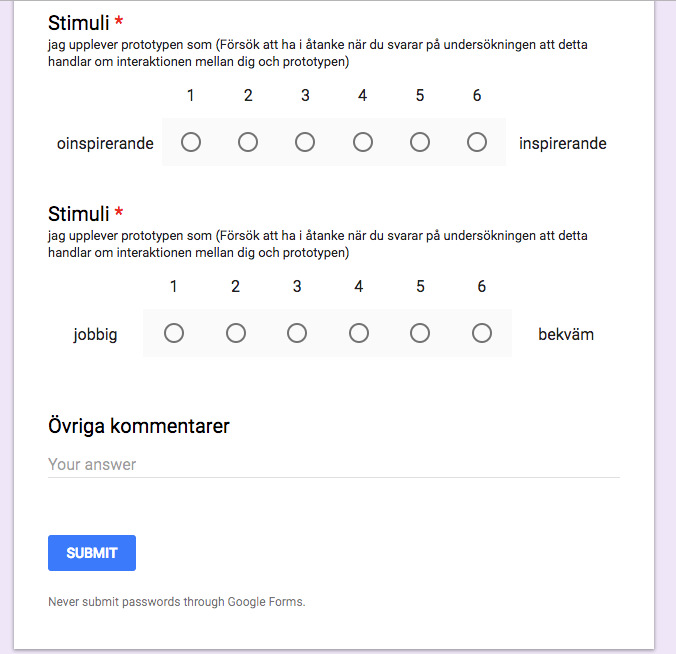
\includegraphics[scale=0.75]{form5.png}
  \captionsetup{justification=centering,margin=2cm}
  \caption{Enkätundersökning}
 \end{figure} 


\end{document}
